\chapter{Implementation and Experimental Setup}

This chapter describes the complete end-to-end implementation of RE-TabSyn, covering pipeline architecture, data preprocessing, model configurations, training procedures, and the generation protocol. Every choice is explained in sufficient detail to allow replication.

All experiments were conducted using Python 3.13.5 with PyTorch 2.9.1 as the deep learning framework, on a MacBook Air equipped with an Apple M3 chip and 16 GB of unified RAM running macOS 26.3.1. Supporting libraries include NumPy 2.3.5, Pandas 2.3.3, scikit-learn 1.7.2, and XGBoost 3.1.2. The full software stack is documented in this chapter, including the rationale for each technology choice.

\section{Experimental Environment}

All experiments were run on a single machine with a fixed hardware and software configuration. This section documents that configuration so results can be reproduced precisely. Hardware and software choices are explained together with the rationale for each.

\subsection{Hardware}

The Apple M3 chip is a system-on-chip, i.e., SoC, design that integrates the CPU, GPU, and memory onto a single die. The property relevant to this research is \textit{unified memory}: the CPU and GPU share the same 16 GB of RAM rather than maintaining separate memory pools. For deep learning, this removes the bottleneck of copying data between CPU memory and a discrete GPU's dedicated VRAM, which is often the limiting factor in small-to-medium model training workflows. The M3 chip's Neural Engine provides hardware acceleration for matrix multiplication, the core operation in neural network forward and backward passes.

For the model sizes and dataset sizes in this research (datasets up to 45,222 rows, models with up to a few million parameters), the M3 chip provides sufficient computational capacity. The largest training run (RE-TabSyn on Polish Bankruptcy, which has 64 features) completes within a few hours. Larger-scale production deployments would benefit from dedicated GPU hardware, but for research-scale validation the M3 setup is adequate and reproducible on accessible consumer hardware.

\subsection{Software stack}

\textbf{Python 3.13.5} was used as the primary programming language. Python is the standard language for machine learning research due to its extensive ecosystem of scientific computing libraries, readability, and the availability of PyTorch bindings.

\textbf{PyTorch 2.9.1} was chosen as the deep learning framework over alternatives like TensorFlow or JAX for two reasons. First, PyTorch's eager execution model (where operations execute immediately rather than being compiled into a static graph) makes debugging considerably easier: you can inspect intermediate tensors, add print statements, and use standard Python debuggers. For research involving non-standard architectures, this flexibility outweighs the performance benefits of compiled execution. Second, the official implementations of TabSyn and TabDDPM that we use as baselines are both written in PyTorch, ensuring consistency and avoiding potential discrepancies from framework-porting.

\textbf{NumPy 2.3.5} handles numerical array operations outside of PyTorch, including preprocessing steps that operate on CPU arrays before model input and postprocessing steps that convert model outputs back to tabular form.

\textbf{Pandas 2.3.3} handles data loading, inspection, and the initial cleaning of raw CSV files. It provides the DataFrame abstraction that makes working with heterogeneous tabular data natural.

\textbf{scikit-learn 1.7.2} provides the preprocessing transformers (QuantileTransformer, LabelEncoder) and evaluation utilities used throughout the pipeline. Its API design, with \texttt{fit} on training data and \texttt{transform} on both training and test data, prevents data leakage by ensuring that preprocessing statistics are computed only from training data.

\textbf{XGBoost 3.1.2} is used as the downstream classifier in the TSTR evaluation. XGBoost, i.e., eXtreme Gradient Boosting \cite{chen2016xgboost}, is a well-optimized implementation of gradient-boosted decision trees. On tabular classification tasks, XGBoost consistently outperforms or matches deep learning methods, making it the appropriate choice for evaluating whether synthetic data preserves ML-relevant signal. Using a powerful classifier for evaluation rather than a weaker one (like logistic regression) ensures that fidelity differences between synthetic data methods are not masked by the classifier's inability to exploit the training data.

\section{End-to-End Pipeline Architecture}

The implementation of RE-TabSyn covers a complete end-to-end pipeline designed for reliability and reproducibility. Figure~\ref{fig:pipeline_detailed} shows every step from raw data ingestion to the final synthetic output. Figure~\ref{fig:pipeline} provides a complementary high-level view of the sequential flow.

\begin{figure}[!ht]
\centering
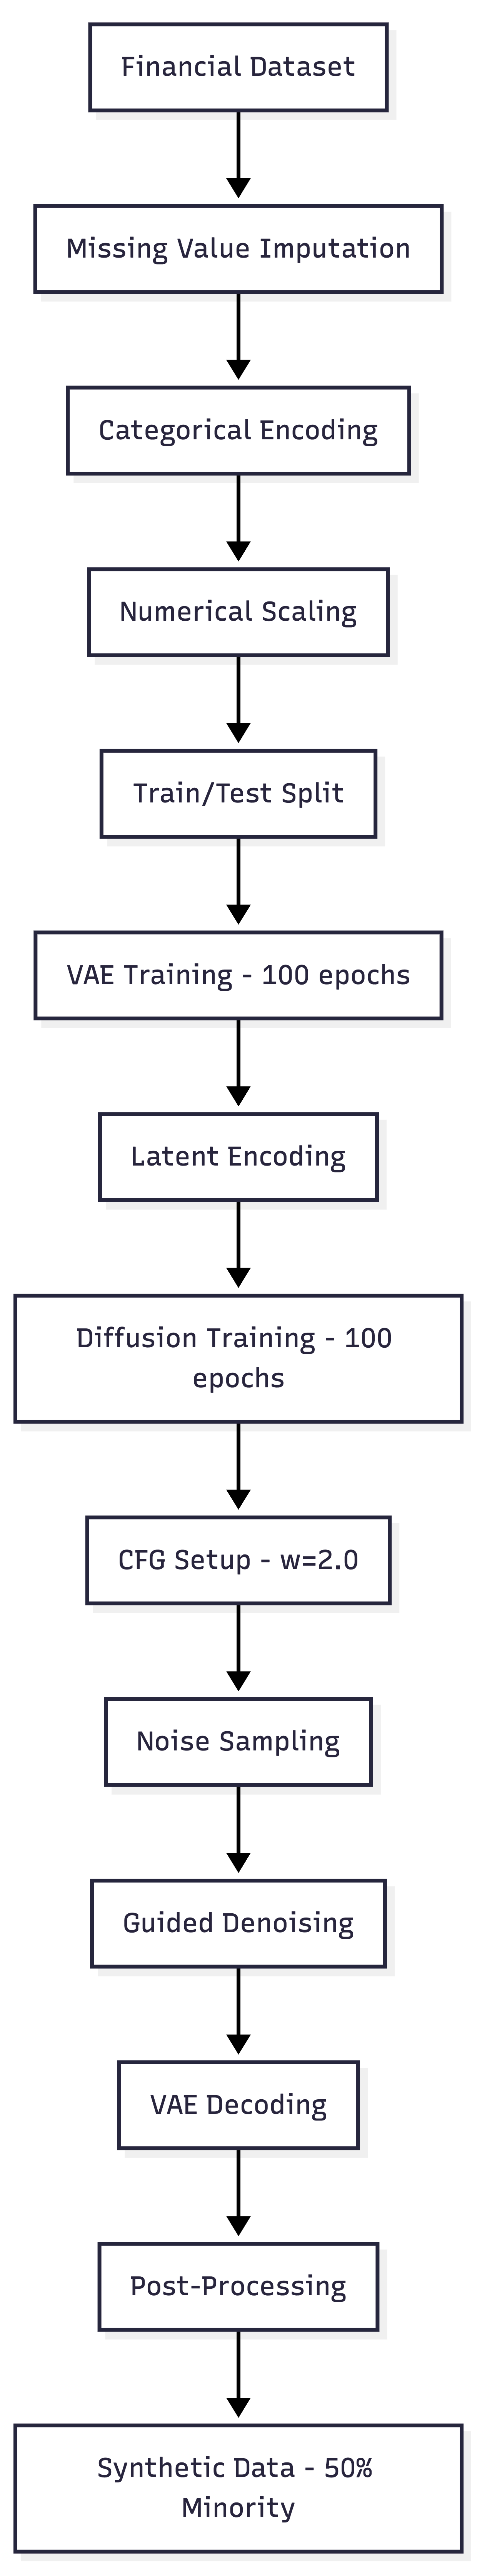
\includegraphics[width=0.45\textwidth]{img/pipeline_detailed.png}
\caption{RE-TabSyn step-by-step pipeline: from raw financial data to balanced synthetic output with 50\% minority.}
\label{fig:pipeline_detailed}
\end{figure}

Each module is independent, receiving a well-defined input and producing a well-defined output. This modularity allows fidelity issues to be traced to a specific stage rather than the system as a whole.

The pipeline consists of five integrated modules:
\begin{enumerate}
    \item \textbf{Data Ingestion Module:} Provides unified access to all six benchmark datasets with automatic download, caching, and versioning. Each dataset is loaded through a standardized interface that identifies numerical columns, categorical columns, and the target variable. This standardization is important: without it, each dataset would require separate ad-hoc preprocessing code, making it impossible to compare results fairly across datasets.

    \item \textbf{Preprocessing Module:} Transforms raw data into model-ready tensors through a sequence of imputation, encoding, and scaling operations (detailed in Section~\ref{sec:preprocessing}). All preprocessing transformers are fit on the training split only and applied to both training and test splits, preventing any information from the test set from influencing the preprocessing parameters.

    \item \textbf{Model Training Pipeline:} Implements the two-phase training protocol: first training the VAE encoder-decoder to convergence, then training the Latent Diffusion Model with Classifier-Free Guidance on frozen VAE latent representations. Freezing the VAE during diffusion training is a deliberate choice: it ensures that the latent space geometry does not shift during diffusion training, which would invalidate the already-learned encoder and require expensive retraining.

    \item \textbf{Generation Module:} Performs latent sampling, CFG-guided denoising, VAE decoding, and reverse transformation to produce synthetic tabular data in the original feature space. The output is a Pandas DataFrame in the same format as the original data, ready for downstream use without any additional processing.

    \item \textbf{Evaluation Module:} Computes a full suite of statistical fidelity, machine learning utility, and privacy metrics, generating both numerical results and visualizations. All metrics are computed three times (once per random seed) and reported as mean and standard deviation.
\end{enumerate}

\begin{figure}[!ht]
\centering
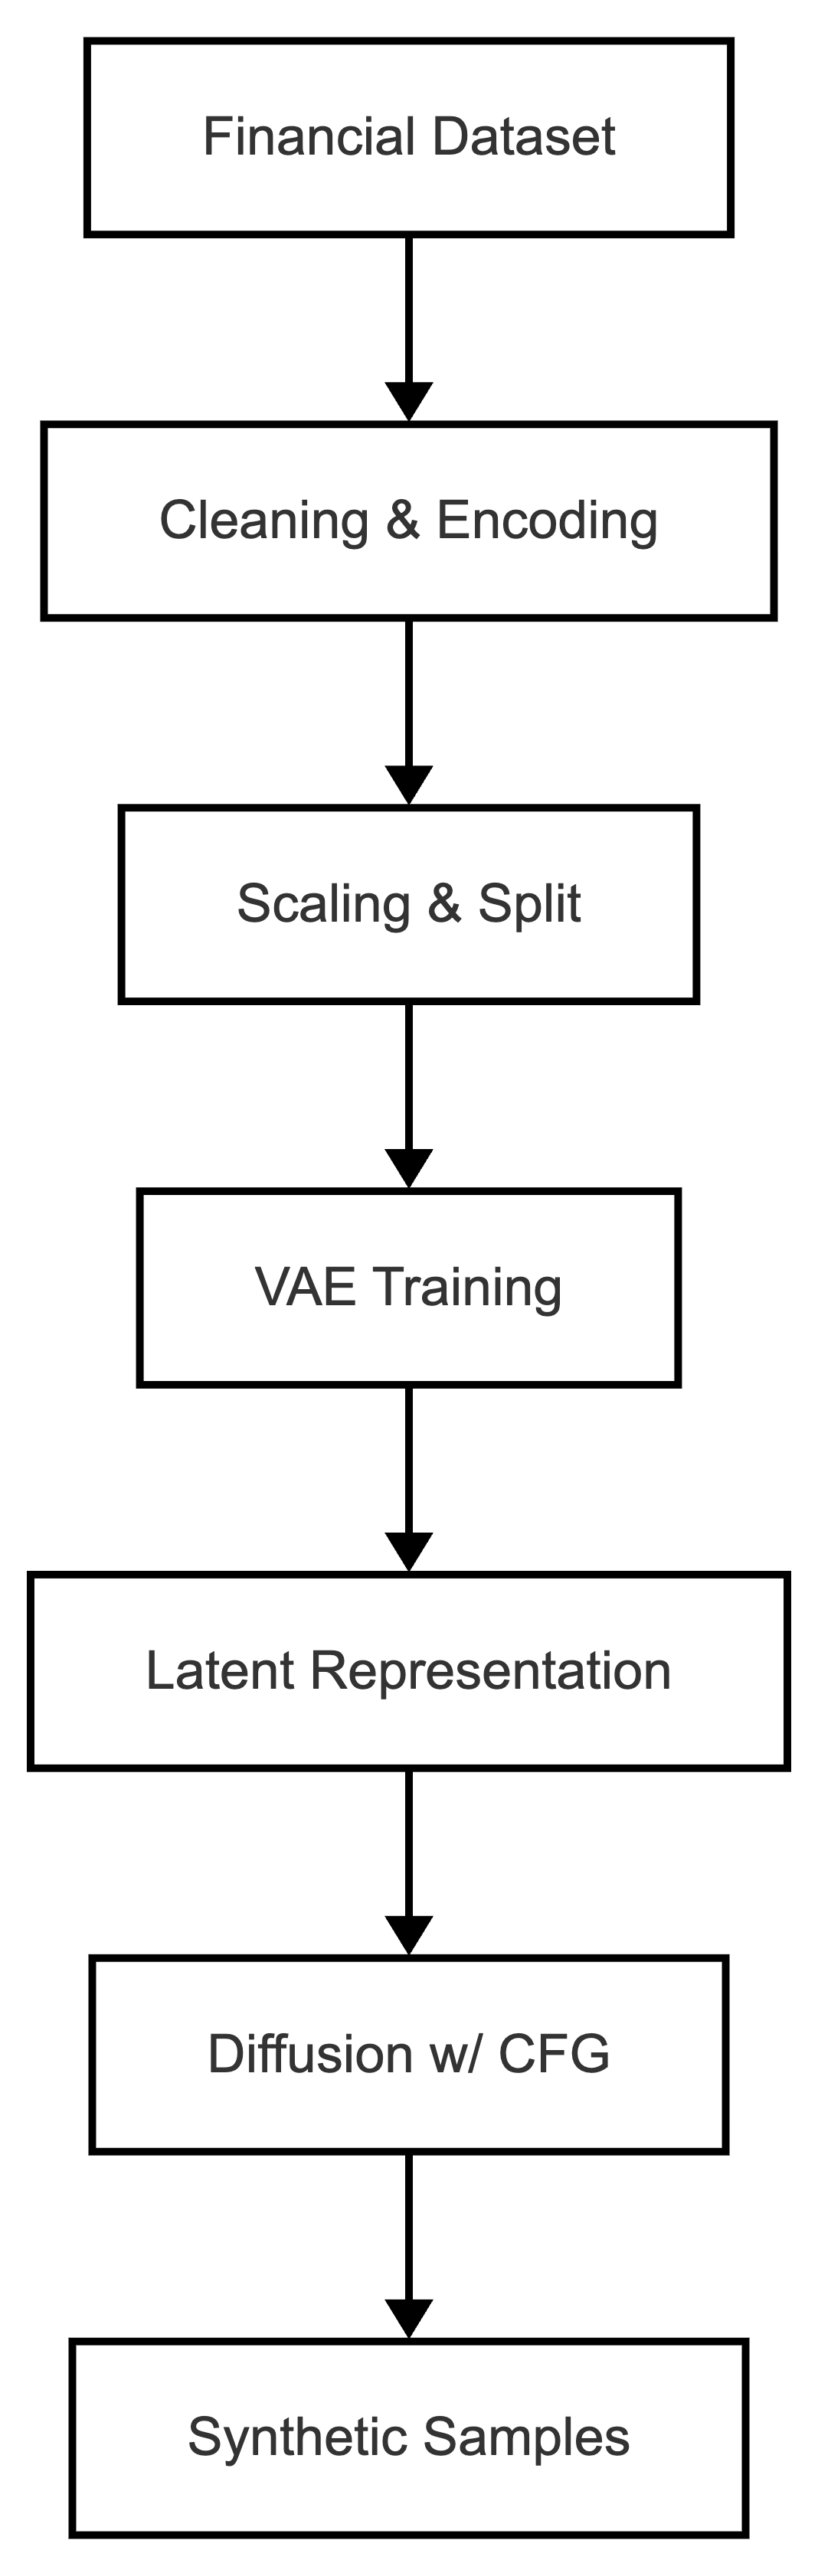
\includegraphics[width=0.4\textwidth]{img/pipeline.png}
\caption{High-level RE-TabSyn pipeline: preprocess, train VAE, train diffusion with CFG, generate synthetic data.}
\label{fig:pipeline}
\end{figure}

\section{Data Preprocessing}
\label{sec:preprocessing}

Preprocessing is where many tabular synthesis attempts fail. A model cannot recover structure that preprocessing has distorted, regardless of architectural complexity.

The preprocessing pipeline for RE-TabSyn follows four steps applied in order: (1) missing value imputation, (2) feature encoding, (3) feature scaling, and (4) train-test splitting. Each step is fit on training data only. Figure~\ref{fig:preprocessing_flow} shows the full flow from raw CSV to the final train/test splits.

\begin{figure}[!ht]
\centering
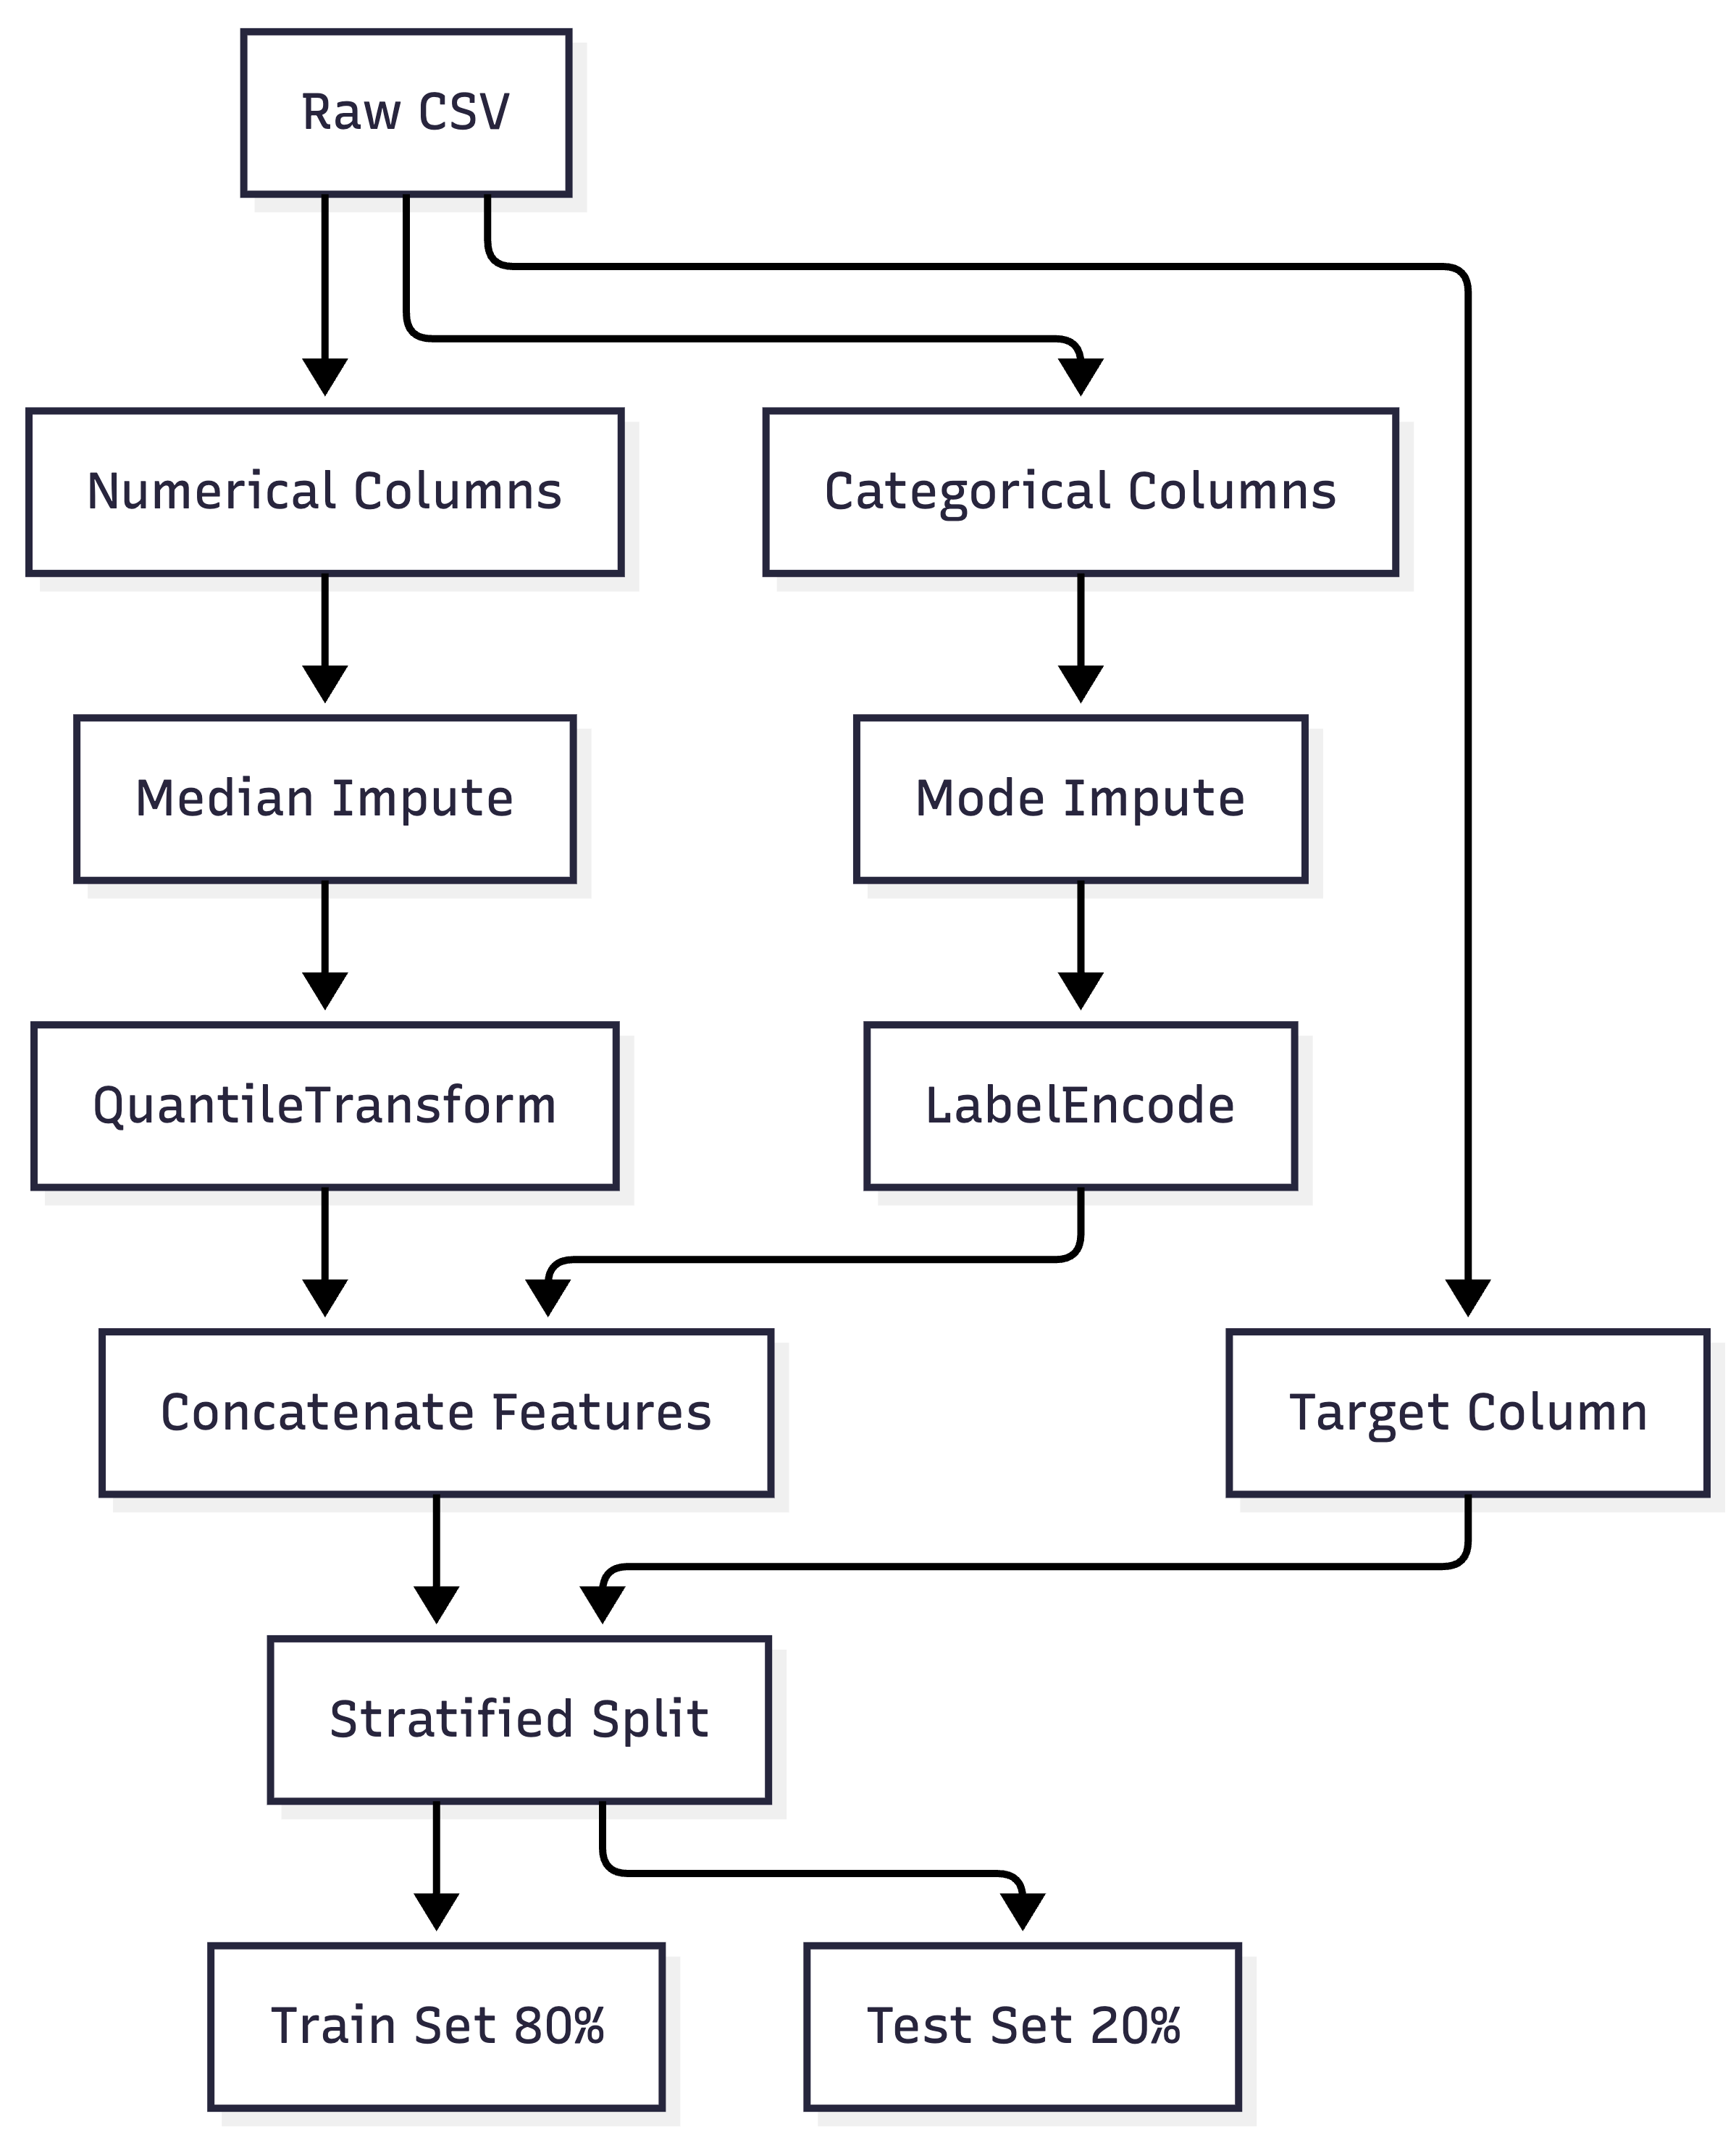
\includegraphics[width=0.55\textwidth]{img/preprocessing_flow.png}
\caption{Preprocessing flow: separate numerical (median impute, QuantileTransform) and categorical (mode impute, label encode) branches, merged then split 80/20 by stratified sampling.}
\label{fig:preprocessing_flow}
\end{figure}

\subsection{Missing value handling}

Missing values are handled through a two-strategy approach, with the choice depending on the feature type:

\textbf{Numerical columns} have missing values imputed with the column median. The median is preferred over the mean for financial data because financial distributions are often heavily skewed: a small number of very high incomes or very large transactions can pull the mean far from where most of the data lies. The median, defined as the 50th percentile, is resistant to these outliers and provides a more representative central value. For example, if a household income column has values ranging from \$20K to \$5M, the mean might be \$80K (inflated by a few ultra-high earners) while the median is \$52K (reflecting where the bulk of the population actually sits). Imputing with \$52K is more likely to produce realistic-looking records than imputing with \$80K.

\textbf{Categorical columns} have missing values imputed with the column mode (the most frequently occurring category). The rationale is that the mode represents the typical case for that column: if 60\% of applicants list ``employed'' as their employment status and the field is missing, ``employed'' is the most plausible fill. An alternative approach, treating missingness as a distinct category (for instance, ``employment\_status\_unknown''), is also supported and can be useful when the pattern of missingness itself carries information (e.g., fields that are left blank on loan applications may correlate with certain applicant behaviors).

\subsection{Feature encoding and scaling}

\textbf{Numerical Features} are transformed using a Quantile Transformer that maps arbitrary distributions to a standard normal distribution ($\mathcal{N}(0, 1)$). This step addresses a persistent problem with financial data: it is almost never normally distributed.

Consider transaction amounts. Most transactions are for small amounts (groceries, utility bills), while a few are for very large amounts (car purchases, property transactions). The resulting distribution has an extremely long right tail. If we feed this raw distribution into a VAE, the model will spend most of its capacity modelling the common small-transaction case and will poorly represent the rare large-transaction case, which is precisely where fraud and risk events are more likely to occur.

The Quantile Transformer solves this by mapping the entire distribution uniformly onto the $[0, 1]$ interval (quantile normalization) and then applying the inverse normal CDF to produce a standard normal distribution. This transformation is guaranteed to be invertible: given a transformed value, you can exactly recover the original value by applying the inverse transform. The result is that every part of the distribution is given equal representational weight during model training, regardless of how rare or common that region is in the raw data. The Gaussian output also satisfies the VAE's implicit assumption that the input space is roughly continuous and smooth.

\textbf{Categorical Features} are converted using Label Encoding, which maps each category to an integer in $\{0, 1, \ldots, K-1\}$ where $K$ is the number of distinct categories. This might seem surprising: why not use one-hot encoding, which is more common in machine learning?

The answer comes directly from the failure of TabDDPM described in the previous chapter. One-hot encoding of a categorical feature with $K$ categories creates a $K$-dimensional sparse binary vector where exactly one element is 1. When many such features are concatenated, the resulting input vector is very high-dimensional and extremely sparse. For a dataset with 10 categorical features each having 10 categories, one-hot encoding produces a 100-dimensional sparse vector (versus 10 dimensions for label encoding). This high dimensionality causes diffusion models to struggle because the noise added during the forward process creates vectors that are not sparse in the way one-hot vectors are, making the reverse denoising task poorly-conditioned.

Label encoding avoids this explosion in dimensionality. The VAE encoder then learns to embed these integer-encoded categories into continuous latent representations, effectively creating its own learned embeddings for each category. The VAE's encoder is flexible enough to learn whatever embedding is most useful for reconstruction, rather than being constrained to the fixed geometry of one-hot vectors.

\subsection{Benchmark datasets}

Table~\ref{tab:datasets} summarizes the six financial benchmark datasets used in our experiments. Each dataset was selected to represent a distinct sub-domain of financial machine learning, to cover a range of class imbalance severities, and to test the method on both small and large sample sizes.

\begin{table}[!ht]
\centering
\caption{Benchmark Dataset Characteristics}
\label{tab:datasets}
\small
\begin{tabularx}{\textwidth}{|l|c|c|c|c|X|}
\hline
\textbf{Dataset} & \textbf{Samples} & \textbf{Num.} & \textbf{Cat.} & \textbf{Min. \%} & \textbf{Domain} \\
\hline
Adult Income & 45,222 & 6 & 8 & 24.8\% & Income prediction \\
\hline
German Credit & 1,000 & 7 & 13 & 30.0\% & Credit risk \\
\hline
Bank Marketing & 41,188 & 10 & 10 & 11.3\% & Marketing response \\
\hline
Credit Approval & 690 & 6 & 9 & 44.5\% & Credit scoring \\
\hline
Lending Club & 10,000 & 8 & 4 & 20.0\% & Loan default \\
\hline
Polish Bankruptcy & 5,000 & 64 & 0 & 4.8\% & Corporate bankruptcy \\
\hline
\end{tabularx}
\end{table}

Table~\ref{tab:dataset_sources} provides the source, URL, and authenticity information for each dataset.

\begin{table}[!ht]
\centering
\caption{Dataset Sources, Repositories, and Provenance}
\label{tab:dataset_sources}
\small
\begin{tabularx}{\textwidth}{|l|l|>{\footnotesize\raggedright\arraybackslash}X|>{\raggedright\arraybackslash}X|}
\hline
\textbf{Dataset} & \textbf{Repository} & \textbf{URL} & \textbf{Original Source / Creators} \\
\hline
Adult Income & UCI ML Repository & \url{https://archive.ics.uci.edu/dataset/2/adult} & Kohavi \& Becker (1996), U.S. Census Bureau \\
\hline
German Credit & UCI ML Repository & \url{https://archive.ics.uci.edu/dataset/144/statlog+german+credit+data} & Prof.\ H. Hofmann, Universit\"{a}t Hamburg (1994) \\
\hline
Bank Marketing & UCI ML Repository & \url{https://archive.ics.uci.edu/dataset/222/bank+marketing} & Moro, Cortez \& Rita (2014), Portuguese bank records \\
\hline
Credit Approval & UCI ML Repository & \url{https://archive.ics.uci.edu/dataset/27/credit+approval} & J.R.\ Quinlan (1987), anonymised for privacy \\
\hline
Lending Club & Kaggle / LendingClub Corp. & \url{https://www.kaggle.com/datasets/wordsforthewise/lending-club} & LendingClub Corporation (SEC-regulated, publicly traded) \\
\hline
Polish Bankruptcy & UCI ML Repository & \url{https://archive.ics.uci.edu/dataset/365/polish+companies+bankruptcy+data} & Zieba et al.\ (2016), EMIS financial database \\
\hline
\end{tabularx}
\end{table}

All UCI datasets are hosted by the University of California, Irvine, the most widely used public repository for machine learning benchmarks with over 650 curated datasets and peer-reviewed provenance documentation. The Lending Club dataset originates from LendingClub Corporation, a publicly traded US fintech lender (NYSE: LC) subject to SEC and FDIC disclosure requirements; the loan data is drawn from their publicly released statistical filings. All six datasets have been used in multiple peer-reviewed publications, confirming their acceptance as valid benchmarks within the research community.

Figure~\ref{fig:dataset_overview} (Chapter~1) groups the six datasets by their degree of class imbalance, illustrating the range the benchmark covers.

A description of each dataset and the specific reason it was included:

\textbf{Adult Income} \cite{uci_adult} \textbf{(UCI Machine Learning Repository):}
Contains US Census data on 45,222 individuals with features including age, education level, occupation, and weekly working hours. The binary label indicates whether annual income exceeds \$50{,}000. Collected by Ron Kohavi and Barry Becker from the 1994 US Census database.

\textit{Selection rationale:} This is the single largest dataset in the benchmark. At 45,222 samples with a 24.8\% minority ratio, it tests whether RE-TabSyn scales to real-world dataset sizes without performance degradation. The mix of 6 numerical and 8 categorical features represents the kind of heterogeneity common in retail banking customer data. Its presence in the benchmark since 1996 and citation in thousands of studies means results on this dataset can be directly compared with a large body of prior work.

\textbf{German Credit} \cite{uci_german} \textbf{(UCI Machine Learning Repository):}
A credit risk dataset of 1,000 loan applicants from a German bank, classified as good or bad credit risks. Created by Prof.\ Hans Hofmann at Universit\"{a}t Hamburg in 1994. With 13 categorical and only 7 numerical features, it has the highest proportion of categorical attributes in the benchmark.

\textit{Selection rationale:} German Credit tests the most demanding scenario for mixed-type encoding: more categorical features than numerical ones. If the VAE cannot handle predominantly categorical data, this dataset will expose it. At 1,000 records it also represents the data-scarce setting common in niche credit risk domains, where collecting labeled default data over years of observation is expensive and slow. Prior tabular synthesis papers almost universally report results on this dataset, making it a required comparison point.

\textbf{Bank Marketing} \cite{uci_bankmarketing} \textbf{(UCI Machine Learning Repository):}
Records 41,188 direct marketing calls by a Portuguese bank between 2008 and 2013. The binary target indicates whether the contacted client subscribed to a term deposit. Assembled by Moro, Cortez, and Rita for their 2014 study on data-driven marketing prediction.

\textit{Selection rationale:} Marketing conversion datasets have an imbalance structure (11.3\% subscription rate) that is lower than German Credit but higher than Polish Bankruptcy, placing it in the moderate-imbalance band where CFG guidance should provide the clearest improvement. The large dataset size (41,188 rows) pairs with German Credit to test whether results are consistent across small and large datasets. The temporal nature of the data (calls over 5 years) also introduces realistic distribution drift within the dataset, testing robustness.

\textbf{Credit Approval} \cite{uci_creditapproval} \textbf{(UCI Machine Learning Repository):}
The smallest dataset in the benchmark with only 690 records. Features and many values have been anonymised by the original contributor, J.R.\ Quinlan, to protect proprietary credit bureau information. The 44.5\% minority ratio makes it nearly balanced.

\textit{Selection rationale:} Its near-balanced class distribution makes it a stress test in the opposite direction. CFG is designed to boost minority representation, but it must not over-correct and distort an already-balanced dataset. Including Credit Approval checks that RE-TabSyn degrades gracefully when minority boosting is not needed. Its 690 records also represent the smallest realistic training set size for a generative model, testing the lower bound of data requirements.

\textbf{Lending Club Loan Data} \cite{kaggle_lendingclub} \textbf{(Kaggle / LendingClub Corporation):}
Contains application attributes and repayment outcomes for loans issued by LendingClub Corporation, a SEC-registered peer-to-peer lender. The full dataset covers millions of loans; we use a stratified subsample of 10,000 records. Features include debt-to-income ratio, loan grade, employment length, and annual income. The binary label is loan default (minority, 20\%).

\textit{Selection rationale:} This dataset is the only one in the benchmark sourced from a publicly traded company with regulatory disclosure obligations, giving it the strongest real-world provenance of the six. The features (debt-to-income ratio, loan grade, employment length) are the exact variables used in actual underwriting decisions, making performance on this dataset directly relevant to production deployment. The 20\% default rate represents a realistic operational imbalance for consumer lending.

\textbf{Polish Bankruptcy} \cite{uci_polishbankruptcy} \textbf{(UCI Machine Learning Repository):}
Financial ratio data for Polish companies collected from the Emerging Markets Information Service, i.e., EMIS, database, covering the years 2000--2012. Compiled by Zieba et al.\ for their 2016 bankruptcy prediction study. Contains 64 purely numerical financial ratios (current ratio, debt-to-equity, return on assets, and similar) with a 4.8\% bankruptcy rate.

\textit{Selection rationale:} Polish Bankruptcy is the hardest dataset in the benchmark on two dimensions simultaneously. First, the 4.8\% minority ratio is the most extreme imbalance, where class-conditional generation must work hardest. Second, the 64-dimensional purely numerical feature space is the largest in the benchmark, testing whether the 64-dimensional VAE latent space is sufficient to encode all relevant structure. This dataset is where RE-TabSyn's CFG mechanism produces its most visible effect, boosting minority representation from 4.8\% to 47.8\%.

These datasets were selected to cover a wide range of:
\begin{enumerate}
    \item \textbf{Sample sizes:} From 690 (Credit Approval) to 45,222 (Adult Income), testing scalability across two orders of magnitude.
    \item \textbf{Feature compositions:} From purely numerical (Polish Bankruptcy, 64 features) to highly mixed-type (German Credit, 13 categorical and 7 numerical features), testing the mixed-type encoding capability.
    \item \textbf{Imbalance severities:} From near-balanced (Credit Approval at 44.5\%) to extreme imbalance (Polish Bankruptcy at 4.8\%), testing the limits of minority boosting.
    \item \textbf{Financial sub-domains:} Income prediction, credit risk, marketing response, loan performance, and corporate bankruptcy.
\end{enumerate}

\section{Model Configurations}

This section details the architectural configurations and hyperparameters for RE-TabSyn and all baseline methods. All models were configured following their respective authors' recommendations, with adjustments for the financial tabular data domain where necessary.

Table~\ref{tab:hyperparams} provides a consolidated reference of all RE-TabSyn hyperparameters. The rationale for each choice is explained in the subsections that follow.

\begin{table}[!ht]
\centering
\caption{Complete RE-TabSyn Hyperparameter Reference}
\label{tab:hyperparams}
\small
\begin{tabularx}{\textwidth}{|l|l|X|}
\hline
\textbf{Component} & \textbf{Hyperparameter} & \textbf{Value} \\
\hline
\multirow{5}{*}{VAE} & Encoder hidden dims & [256, 128] \\
                     & Decoder hidden dims & [128, 256] \\
                     & Latent dimension $d$ & 64 \\
                     & Activation & ReLU \\
                     & KL weight $\beta$ & 0.1 \\
\hline
\multirow{6}{*}{Diffusion (DiT)} & Number of layers & 4 \\
                                  & Hidden dimension & 256 \\
                                  & Attention heads & 4 \\
                                  & Head dimension & 64 \\
                                  & Timesteps $T$ & 1000 \\
                                  & Noise schedule & Linear \\
                                  & $\beta_1$ (start) & $10^{-4}$ \\
                                  & $\beta_T$ (end) & 0.02 \\
\hline
\multirow{4}{*}{Embeddings} & Time embed dim & 128 \\
                             & Time projection dim & 256 \\
                             & Class vocab size & 3 (0, 1, $\emptyset$) \\
                             & Class embed dim & 256 \\
\hline
\multirow{2}{*}{CFG} & Label dropout $p_{uncond}$ & 0.10 \\
                      & Guidance scale $w$ & 2.0 \\
\hline
\multirow{4}{*}{Training} & Optimiser & Adam \\
                           & Learning rate & $10^{-3}$ \\
                           & Batch size & 256 \\
                           & Epochs per phase & 100 \\
\hline
\multirow{2}{*}{Evaluation} & Train/test split & 80\% / 20\% \\
                              & Random seeds & 42, 123, 456 \\
\hline
\end{tabularx}
\end{table}

\subsection{RE-TabSyn architecture}

The full RE-TabSyn architecture is configured as follows:

\textbf{VAE Encoder:} A Multi-Layer Perceptron, i.e., MLP, with hidden dimensions [256, 128] and ReLU activations. ReLU, i.e., Rectified Linear Unit, was chosen over alternatives like GELU or Tanh because it is computationally cheap, avoids saturation in the middle layers, and provides sufficient non-linearity for the encoding task. The two hidden layers compress the data progressively from the input dimension down to 64. The encoder produces both a mean vector $\mu \in \mathbb{R}^{64}$ and a log-variance vector $\log \sigma^2 \in \mathbb{R}^{64}$ for the 64-dimensional latent space.

\textbf{VAE Decoder:} A mirror architecture [128, 256] with separate output heads. The mirror structure is not strictly required but is a common and effective design: the decoder should roughly invert the encoder, and matching the hidden dimensions provides a natural correspondence. The separate output heads are the distinguishing design choice: a linear projection (followed by the inverse quantile transform) for numerical features, and a softmax projection (followed by argmax) for categorical features. This means each categorical column gets its own softmax head with dimensionality equal to the number of categories in that column, ensuring the decoder can produce a valid probability distribution over all possible values.

\textbf{Diffusion Backbone (DiT):} A Diffusion Transformer architecture with 4 layers, hidden dimension 256, and 4 attention heads (64 dimensions per head). The noise schedule uses $T = 1000$ timesteps with linear $\beta$ variance schedule from $\beta_1 = 10^{-4}$ to $\beta_T = 0.02$. These are the default settings from the original DDPM paper \cite{ho2020ddpm} and have produced consistent results across many subsequent applications.

\textbf{Guidance Parameters:} Label dropout rate $p_{uncond} = 0.10$ during training, meaning 10\% of training samples have their class label replaced with the null token $\emptyset$. Guidance scale $w = 2.0$ during inference, producing near-50\% minority ratios in practice.

\textbf{Embeddings:} Sinusoidal time embeddings with 128-dimensional projection. The sinusoidal embedding maps an integer timestep $t \in \{1, ..., 1000\}$ to a 64-dimensional vector using sine and cosine functions of different frequencies, following Vaswani et al.\ \cite{vaswani2017attention}. These are then projected through a two-layer MLP to a 256-dimensional representation matching the DiT's hidden dimension. Learned class embeddings for 3 tokens (class 0, class 1, null $\emptyset$) are initialized randomly and optimized during training. The null token is treated as a third class, allowing the model to learn a distinct representation for the unconditional case.

\subsection{Baseline configurations}

RE-TabSyn is compared against four established methods. All baseline implementations use their official codebases to ensure fair comparison:

\textbf{CTGAN:} Mode-specific normalization (with variational Gaussian mixture models), a PAC (Packing) discriminator that looks at a pack of 10 samples simultaneously to reduce mode collapse, embedding dimension 128 for categorical features, generator and discriminator hidden dimensions both [256, 256], batch size 500, trained for 100 epochs. The PAC discriminator is a specific improvement to the standard GAN discriminator that helps detect mode collapse by comparing batches of generated samples. Implemented via the SDV (Synthetic Data Vault) library.

\textbf{TVAE:} Standard VAE with CTGAN-compatible tabular preprocessing (same mode-specific normalization), embedding dimension 128, encoder and decoder hidden dimensions both [128, 128], trained for 100 epochs with the default ELBO objective. Implemented via the SDV library.

\textbf{TabDDPM:} Gaussian diffusion for numerical features, multinomial diffusion for categorical features, MLP backbone (not Transformer) with hidden dimensions [256, 256, 256], 1,000 diffusion steps, trained for 100 epochs. The MLP backbone is the original paper's design choice; it does not include self-attention, which is one reason it cannot capture complex inter-feature dependencies as well as the DiT. Implemented from the official repository by Kotelnikov et al.\ \cite{kotelnikov2023tabddpm}.

\textbf{TabSyn:} VAE with a Transformer-based latent diffusion model, without CFG. TabSyn's VAE uses a more complex architecture than RE-TabSyn's (it processes each feature through a separate tokenizer before encoding), and its diffusion backbone is also Transformer-based. This is the highest-fidelity tabular synthesis method in the literature at the time of this work. Implemented from the official repository by Zhang et al.\ \cite{zhang2024tabsyn}.

\subsection{Method comparison at a glance}

Table~\ref{tab:method_comparison} summarises the architectural properties of all five methods side by side, showing where RE-TabSyn sits relative to the alternatives and why each architectural choice differs.

\begin{table}[!ht]
\centering
\caption{Architectural Comparison Across All Methods}
\label{tab:method_comparison}
\small
\begin{tabularx}{\textwidth}{|l|C|C|C|C|C|}
\hline
\textbf{Property} & \textbf{CTGAN} & \textbf{TVAE} & \textbf{TabDDPM} & \textbf{TabSyn} & \textbf{RE-TabSyn} \\
\hline
Framework & GAN & VAE & Diffusion & VAE + Diffusion & VAE + Diffusion + CFG \\
\hline
Generative model & Generator & Decoder & MLP diffusion & DiT diffusion & DiT diffusion \\
\hline
Latent space & No & Yes (128-d) & No & Yes (learned) & Yes (64-d Gaussian) \\
\hline
Handles mixed types & Yes (mode norm.) & Yes (mode norm.) & Poor & Yes & Yes \\
\hline
Minority class control & No & No & No & No & Yes (CFG, $w$) \\
\hline
Class conditioning & No & No & No & No & Yes \\
\hline
Training phases & 1 & 1 & 1 & 2 & 2 \\
\hline
Fast sampling possible & N/A & N/A & DDIM & DDIM & DDIM \\
\hline
Formal DP support & No & No & No & No & Planned (Opacus) \\
\hline
\end{tabularx}
\end{table}

The table confirms one structural fact: RE-TabSyn is the only method among the five that offers minority class control. Every other method generates data according to whatever class distribution exists in the training data. If fraud is 5\% of the training set, every other method will generate fraud 5\% of the time. RE-TabSyn can change this at inference time, with no retraining.

\section{Training Procedures}

Training proceeds in two distinct, sequential phases. The two-phase structure decouples the representation learning problem, i.e., VAE, from the generative modeling problem, i.e., diffusion, allowing each component to be optimized independently. Figure~\ref{fig:two_phase_training} shows the structure of both phases.

\begin{figure}[!ht]
\centering
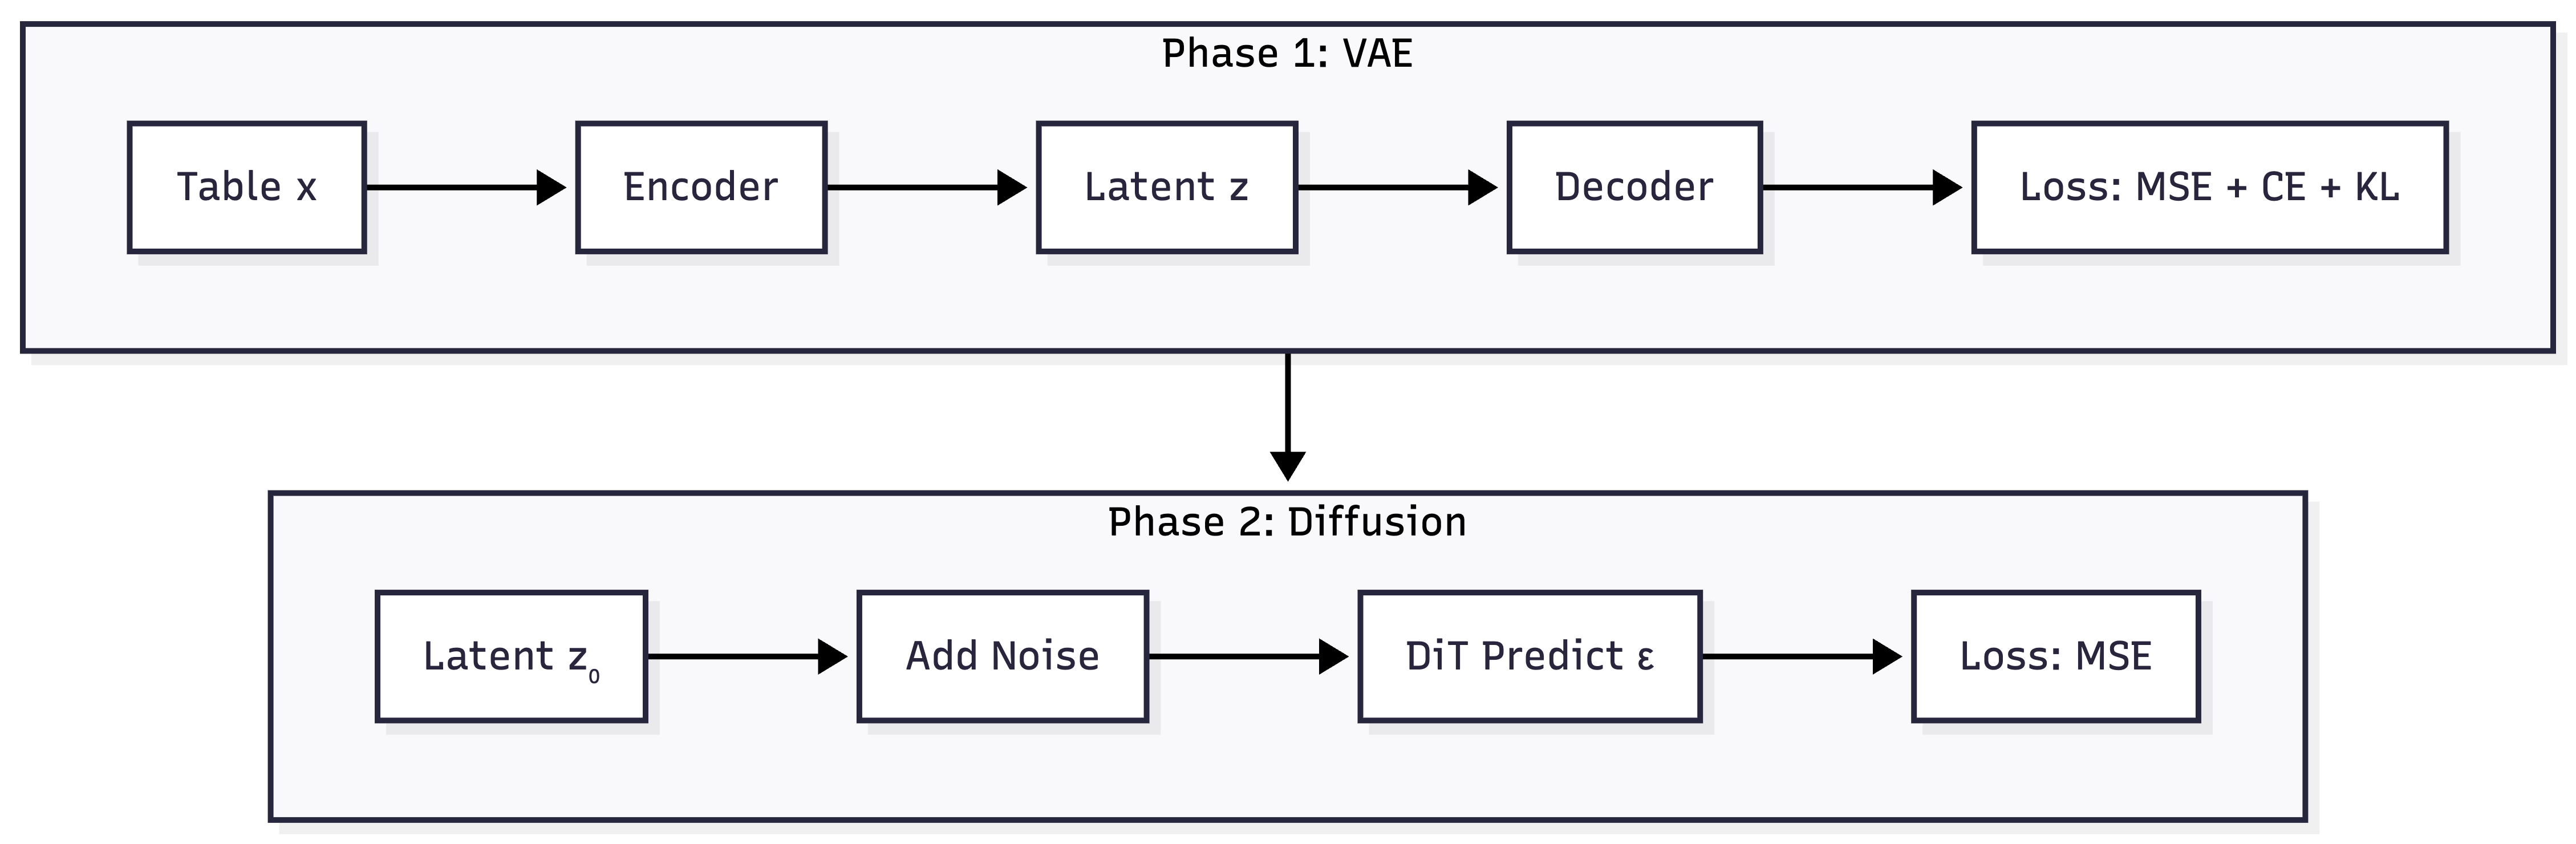
\includegraphics[width=\textwidth]{img/two_phase_training.png}
\caption{Two-phase training: Phase 1 trains the VAE (MSE + CE + KL loss); Phase 2 freezes the VAE and trains the diffusion model (MSE noise prediction).}
\label{fig:two_phase_training}
\end{figure}

\textbf{Phase 1 -- VAE Training (Epochs 1--100):}

\begin{enumerate}
    \item Raw data is preprocessed as described in Section~\ref{sec:preprocessing} and split into training (80\%) and test (20\%) sets. The 80/20 split is standard in machine learning practice. The test set is held out entirely during model training and used only for evaluation.

    \item The VAE is trained to minimize the combined loss: $\mathcal{L}_{VAE} = \mathcal{L}_{MSE} + \mathcal{L}_{CE} + 0.1 \cdot \mathcal{L}_{KL}$. The loss is computed on the training set and the weights are updated using gradient descent. No data augmentation is applied during VAE training.

    \item The KL weight $\beta = 0.1$ is fixed (not annealed). Some VAE training protocols gradually increase $\beta$ from 0 to its final value over the course of training (``KL annealing''), which can help avoid posterior collapse early in training when the reconstruction loss dominates. We found that a fixed $\beta = 0.1$ achieves stable training without collapse across all six datasets, avoiding the additional hyperparameter of the annealing schedule.

    \item Adam optimizer \cite{kingma2015adam} is used with learning rate $10^{-3}$ and default momentum parameters ($\beta_1 = 0.9$, $\beta_2 = 0.999$). Adam is the standard choice for VAE training because it adapts the learning rate per parameter, handling the different scales of numerical and categorical features gracefully. Batch size 256 provides a good balance between gradient noise (smaller batches provide noisier but more frequent updates) and computational efficiency.

    \item Training converges when reconstruction loss stabilizes, typically within 50--80 epochs. The training loop monitors the validation loss (on the held-out 20\% of training data) and saves the model checkpoint at each epoch. The final model used for latent encoding is the checkpoint with the lowest validation loss.
\end{enumerate}

\begin{figure}[!ht]
\centering
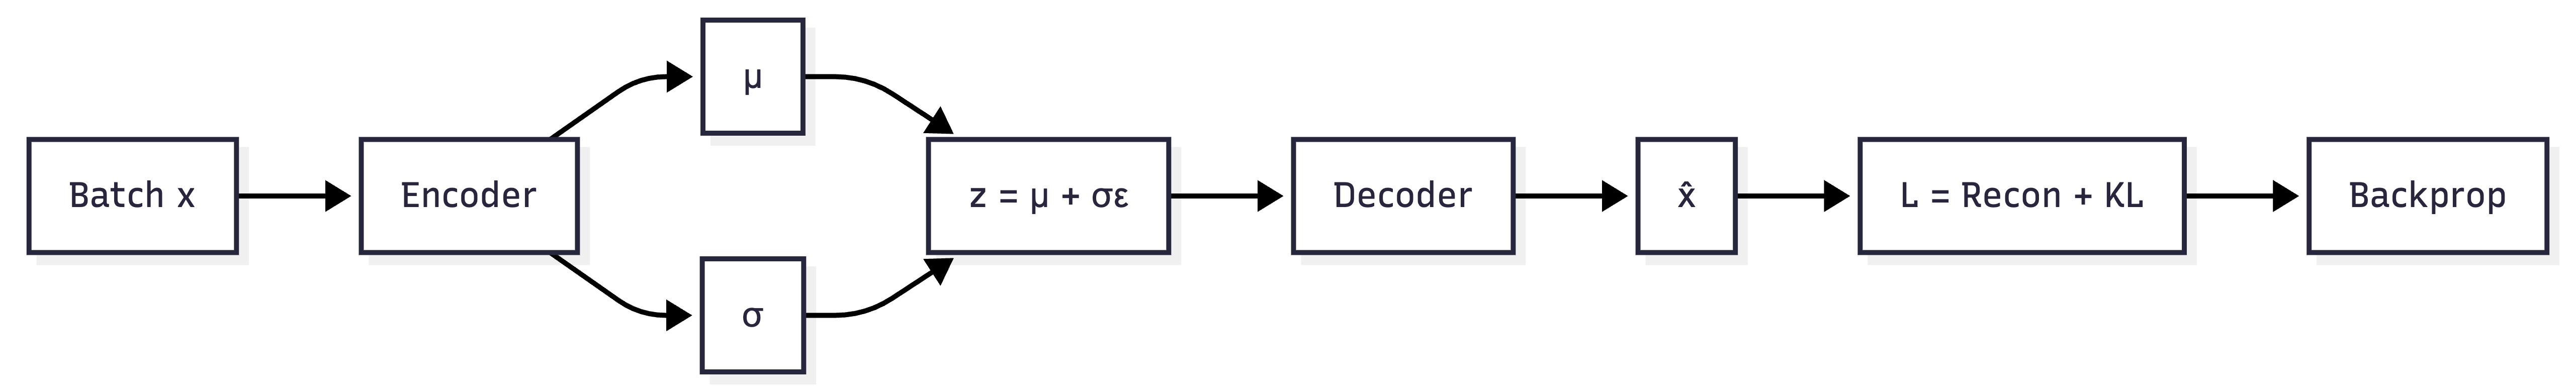
\includegraphics[width=\textwidth]{img/vae_training_loop.png}
\caption{VAE training loop: encode to $(\mu, \sigma)$, reparameterise to $\mathbf{z}$, decode to $\hat{\mathbf{x}}$, backpropagate reconstruction + KL loss.}
\label{fig:vae_training_loop}
\end{figure}

\textbf{Phase 2 -- Diffusion Training (Epochs 1--100):}

\begin{enumerate}
    \item VAE weights are frozen. Freezing is necessary: if the VAE continued training during Phase 2, the latent representations of training data would shift, invalidating the latent codes that the diffusion model has already learned to model. Freezing ensures the latent space is stable throughout Phase 2.

    \item All training data is encoded into the 64-dimensional latent space using the frozen VAE encoder. This encoding step is done once, before training begins, and the resulting latent vectors are cached. This avoids the computational cost of re-encoding the training data at every training step.

    \item For each training step, the following operations are performed: a random timestep $t \sim \mathcal{U}(1, 1000)$ is sampled uniformly; Gaussian noise $\epsilon \sim \mathcal{N}(0, I)$ is sampled; with probability $p_{uncond} = 0.10$, the class label $y$ for this sample is replaced with the null token $\emptyset$; the noisy latent $\mathbf{z}_t = \sqrt{\bar{\alpha}_t}\mathbf{z}_0 + \sqrt{1-\bar{\alpha}_t}\epsilon$ is computed; the DiT predicts $\hat{\epsilon} = \epsilon_\theta(\mathbf{z}_t, t, y)$; and the MSE loss $\|\epsilon - \hat{\epsilon}\|^2$ is backpropagated.

    \item Adam optimizer with the same learning rate $10^{-3}$ and batch size 256 as Phase 1. Using the same optimizer settings for both phases simplifies the hyperparameter search.

    \item All experiments are run with three random seeds (42, 123, 456) to assess result variance. Each seed controls the random initialization of all model weights, the random sampling of timesteps and noise during training, and the random ordering of training batches. Reporting mean and standard deviation across three seeds confirms that the findings are not artifacts of a single initialization.
\end{enumerate}

\begin{figure}[!ht]
\centering
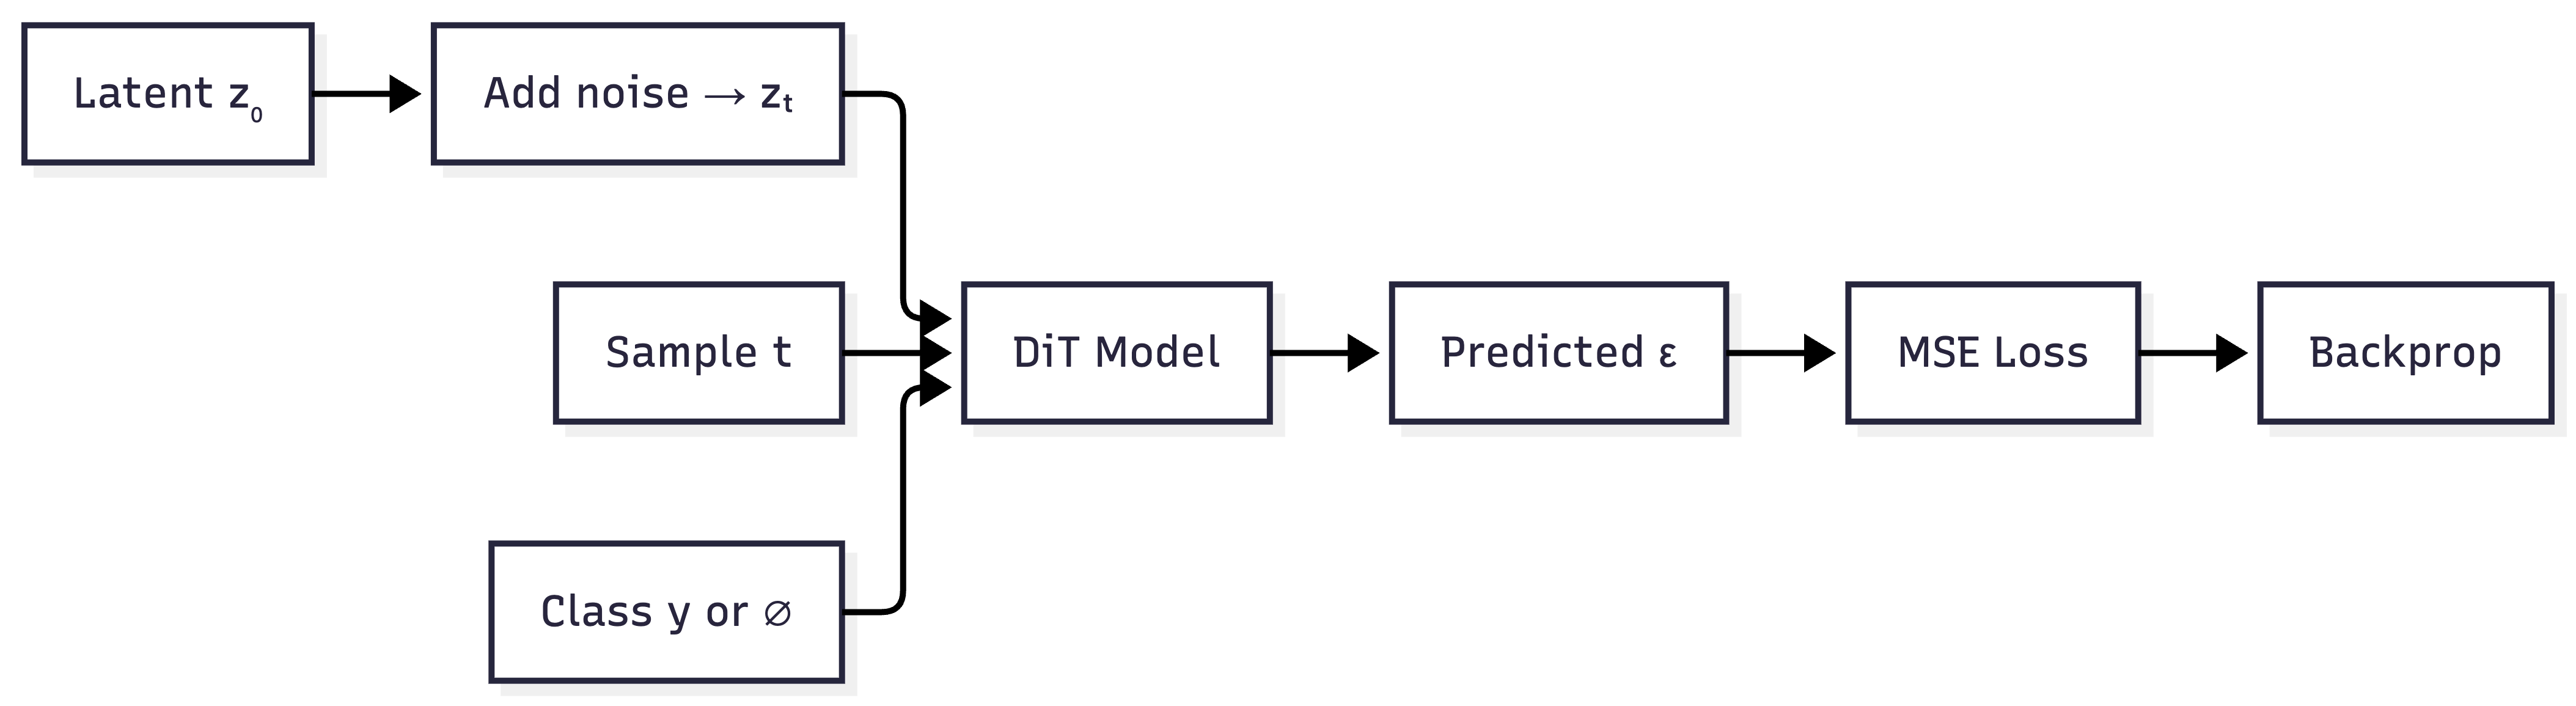
\includegraphics[width=\textwidth]{img/diffusion_training_loop.png}
\caption{Diffusion training loop: noise frozen latent $\mathbf{z}_0$, predict noise $\hat{\epsilon}$ with DiT, backpropagate MSE loss.}
\label{fig:diffusion_training_loop}
\end{figure}

\section{Synthetic Data Generation Procedure}

Generation with RE-TabSyn follows a structured four-step protocol. Once trained, the model can generate any number of synthetic samples with any desired minority ratio without retraining.

\textbf{Step 1 -- Latent Initialization:} Sample $N$ initial noise vectors from $\mathcal{N}(0, I)$ in the 64-dimensional latent space. These are pure random noise vectors, which are the starting point of the reverse diffusion process. To generate balanced data with 50\% minority representation, half of the $N$ samples are assigned class label $y = 1$ and half are assigned $y = 0$. The split can be adjusted to generate any desired ratio: to get 30\% minority, assign 30\% of samples $y = 1$ and 70\% $y = 0$.

\textbf{Step 2 -- CFG-Guided Denoising:} For each of the $T = 1000$ reverse diffusion steps (iterating from $t = T$ down to $t = 1$). Figure~\ref{fig:cfg_denoising_step} shows the two-pass structure of each step:
\begin{enumerate}
    \item Compute the conditional noise prediction: $\epsilon_{cond} = \epsilon_\theta(\mathbf{z}_t, t, y)$. This is a forward pass through the DiT with the class label.
    \item Compute the unconditional noise prediction: $\epsilon_{uncond} = \epsilon_\theta(\mathbf{z}_t, t, \emptyset)$. This is a second forward pass through the same DiT with the null token.
    \item Apply CFG: $\tilde{\epsilon} = \epsilon_{uncond} + w \cdot (\epsilon_{cond} - \epsilon_{uncond})$ with $w = 2.0$.
    \item Update the latent: $\mathbf{z}_{t-1} = f(\mathbf{z}_t, \tilde{\epsilon}, t)$ using the DDPM reverse step formula.
\end{enumerate}

\begin{figure}[!ht]
\centering
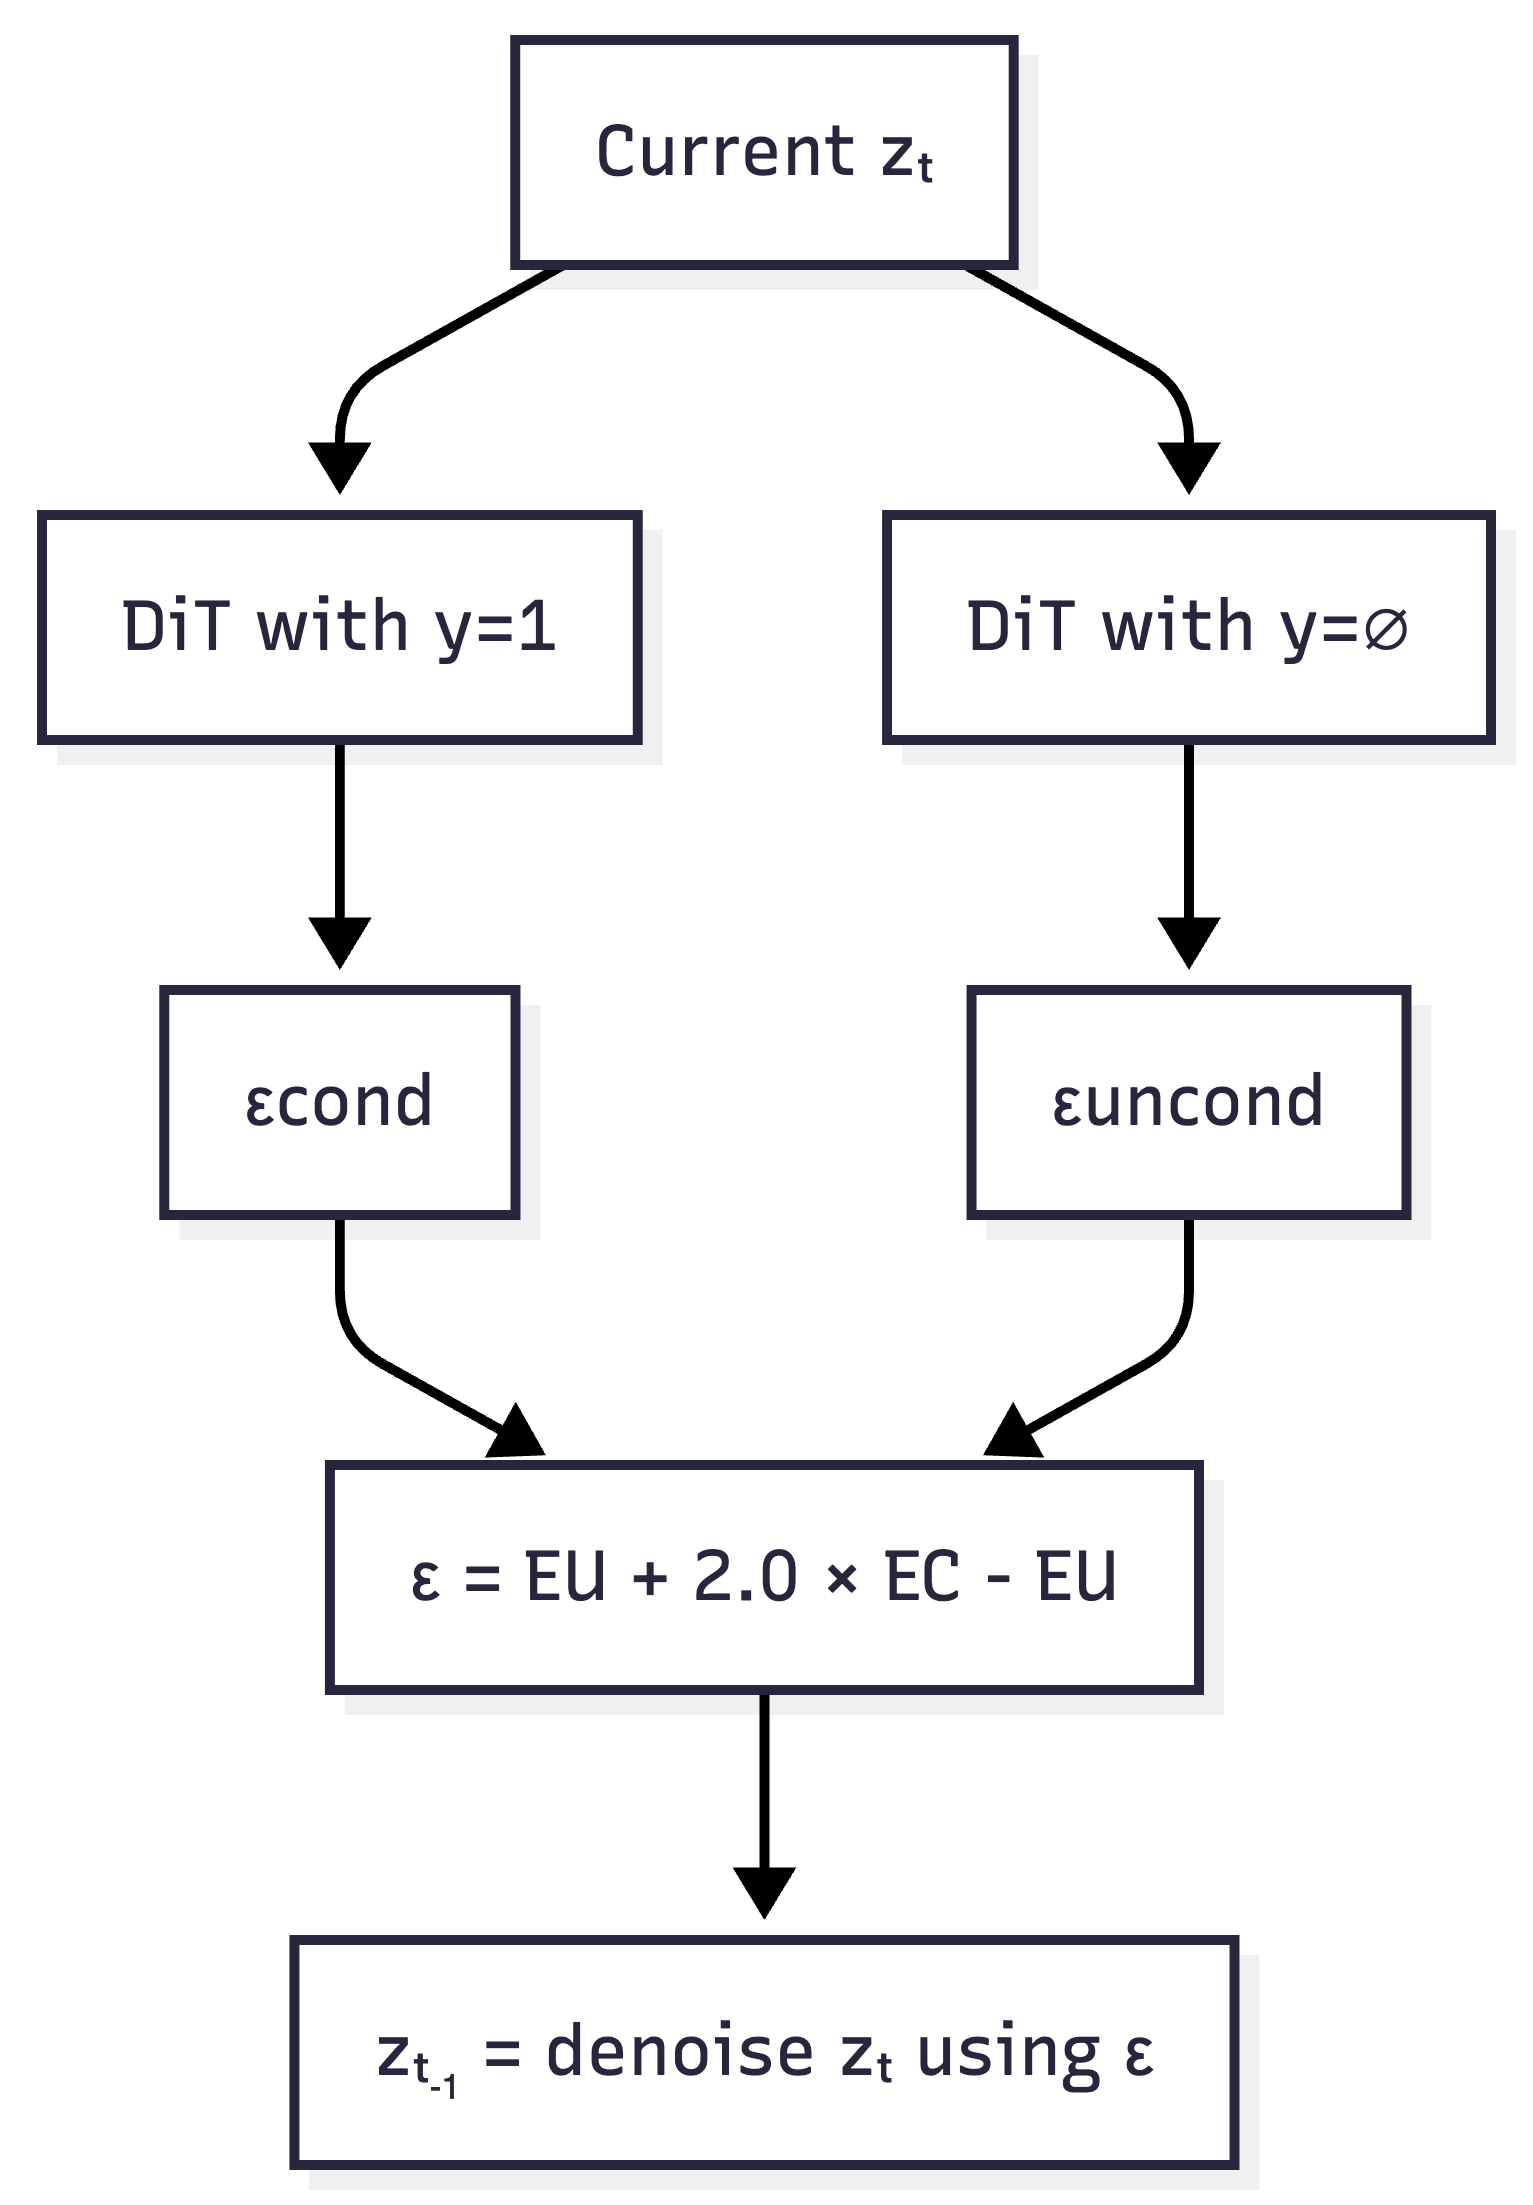
\includegraphics[width=0.80\textwidth]{img/cfg_denoising_step.png}
\caption{Single CFG denoising step: two DiT passes (conditional and unconditional) blended with $w=2.0$ to produce $\mathbf{z}_{t-1}$.}
\label{fig:cfg_denoising_step}
\end{figure}

This procedure requires two forward passes through the DiT per denoising step (one conditional, one unconditional), making CFG generation approximately twice as slow as unconditional generation. For generating 1,000 synthetic samples, this amounts to 2,000,000 DiT forward passes in total ($2 \times 1000 \text{ steps} \times 1000 \text{ samples}$). On the M3 chip, this takes roughly a few minutes per dataset, which is acceptable for research use. Production deployments could accelerate this using fast sampling schedules like DDIM \cite{ho2020ddpm}, which achieves comparable quality in as few as 50 steps.

\textbf{Step 3 -- VAE Decoding:} Pass the denoised latent vectors $\mathbf{z}_0$ (the output of Step 2 after all 1000 denoising steps) through the frozen VAE decoder to reconstruct tabular features.

Numerical features are produced directly from the decoder's linear output heads as real-valued numbers in the transformed (Gaussian) space. Categorical features are obtained via argmax over the softmax probabilities from each categorical output head: the category with the highest predicted probability is selected. This argmax step is the only non-differentiable operation in the entire pipeline, and it occurs only during generation (not during training), so it does not create any training issues.

\textbf{Step 4 -- Reverse Transformation:} Apply the inverse preprocessing pipeline to convert model outputs back to the original feature space. Numerical features are mapped from the Gaussian $\mathcal{N}(0,1)$ representation back to the original distribution via the Inverse Quantile Transformer — an exact inverse that preserves percentile rank. Categorical features are recovered by Inverse Label Encoding, mapping integers back to their original string values (e.g., 2 maps back to ``self-employed'').

The result is a Pandas DataFrame in the original feature space, matching the format of the real data exactly. It can be used directly for downstream machine learning tasks without any additional processing.

\section{Evaluation Framework}

Our evaluation follows the three-pillar framework illustrated in Figure~\ref{fig:evaluation_framework}.

\begin{figure}[!ht]
\centering
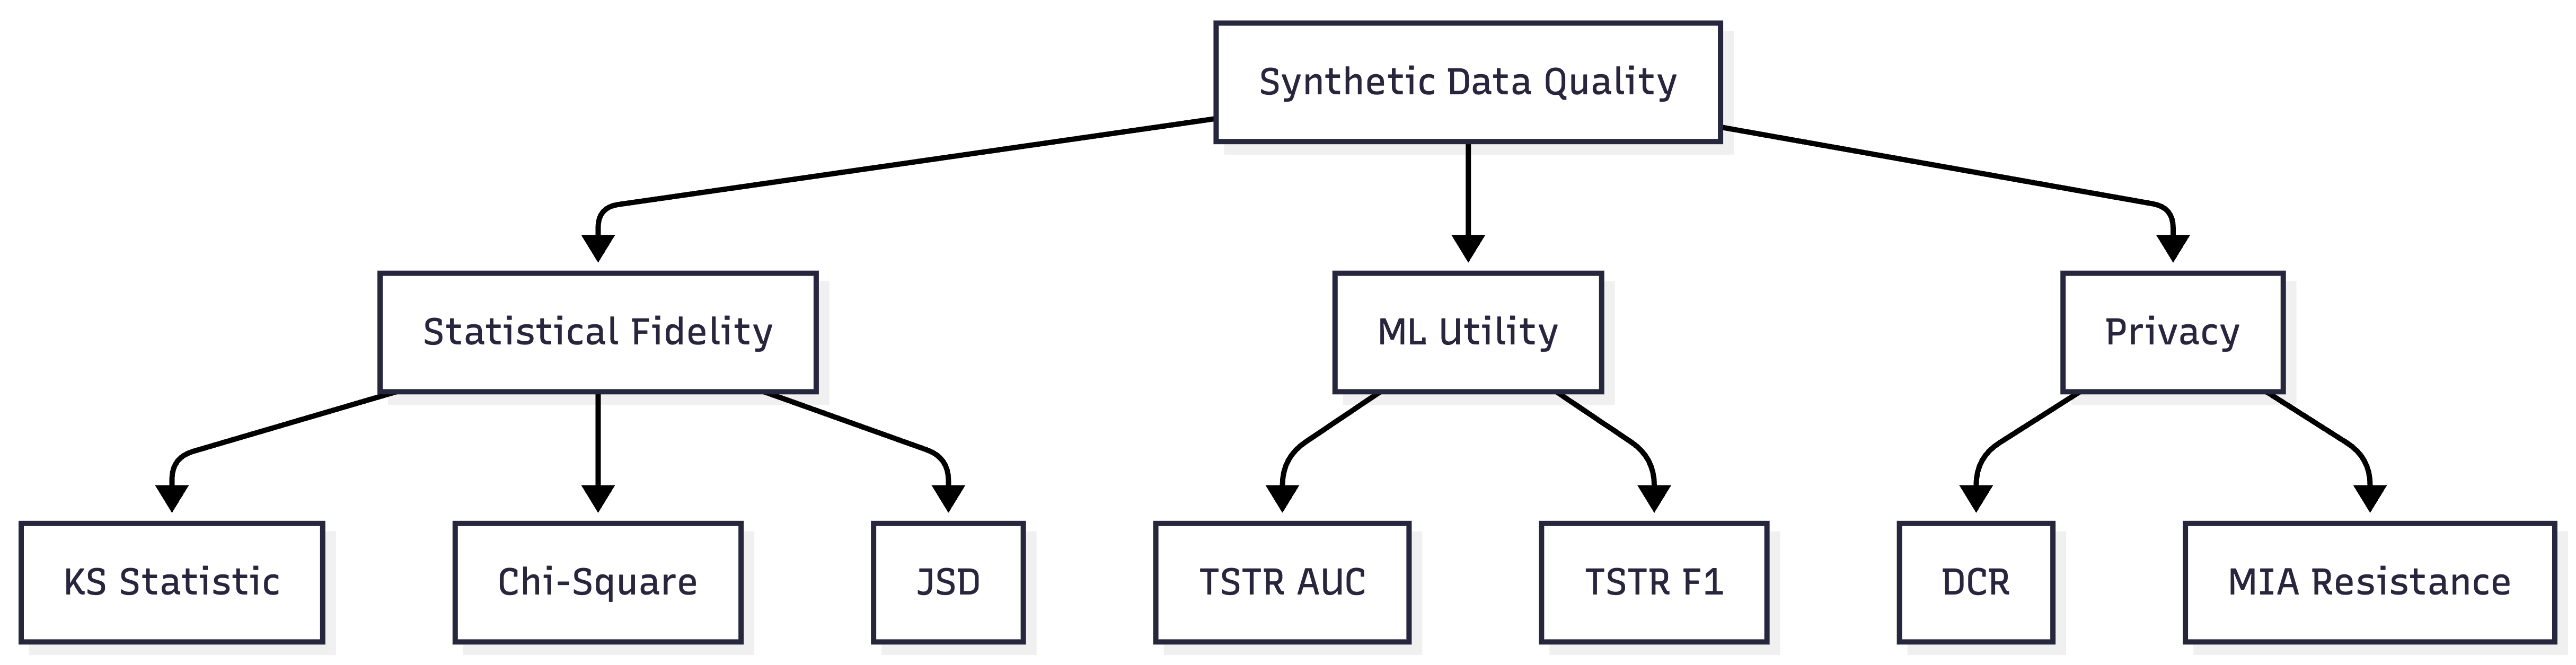
\includegraphics[width=\textwidth]{img/evaluation_framework.png}
\caption{Three-pillar evaluation framework: statistical fidelity (KS, Chi-Square, JSD), ML utility (TSTR AUC, F1), and privacy (DCR, MIA).}
\label{fig:evaluation_framework}
\end{figure}

\subsection{Pillar 1: Statistical fidelity}

Statistical fidelity measures how closely the marginal and joint distributions of synthetic data match those of real data. Two metrics are used.

\textbf{Kolmogorov-Smirnov, i.e., KS, Statistic} \cite{massey1951ks}: For each numerical column, compute the maximum absolute difference between the empirical cumulative distribution functions (CDFs) of the real and synthetic data:
\[
D_{KS} = \sup_x |F_{real}(x) - F_{synth}(x)|
\]
where $F_{real}$ and $F_{synth}$ are the empirical CDFs of the real and synthetic column values respectively. Values range from 0 (identical distributions) to 1 (completely different). We report the average KS across all numerical columns. The KS test is non-parametric: it makes no assumptions about the shape of the distribution and detects differences anywhere in the distribution, not just in the mean or variance.

\textbf{Correlation Preservation:} Compute the $d \times d$ pairwise Pearson correlation matrices for the real and synthetic data (where $d$ is the number of features). Report the mean absolute difference between corresponding entries:
\[
\text{Corr Error} = \frac{1}{d^2} \sum_{i,j} |r_{ij}^{real} - r_{ij}^{synth}|
\]
Lower values indicate better preservation of inter-feature relationships. This captures a dimension that the KS statistic misses: two synthetic datasets could have identical marginal distributions but completely different correlation structures, making them unsuitable for downstream modeling despite appearing similar column-by-column.

\subsection{Pillar 2: Machine learning utility}

\begin{figure}[!ht]
\centering
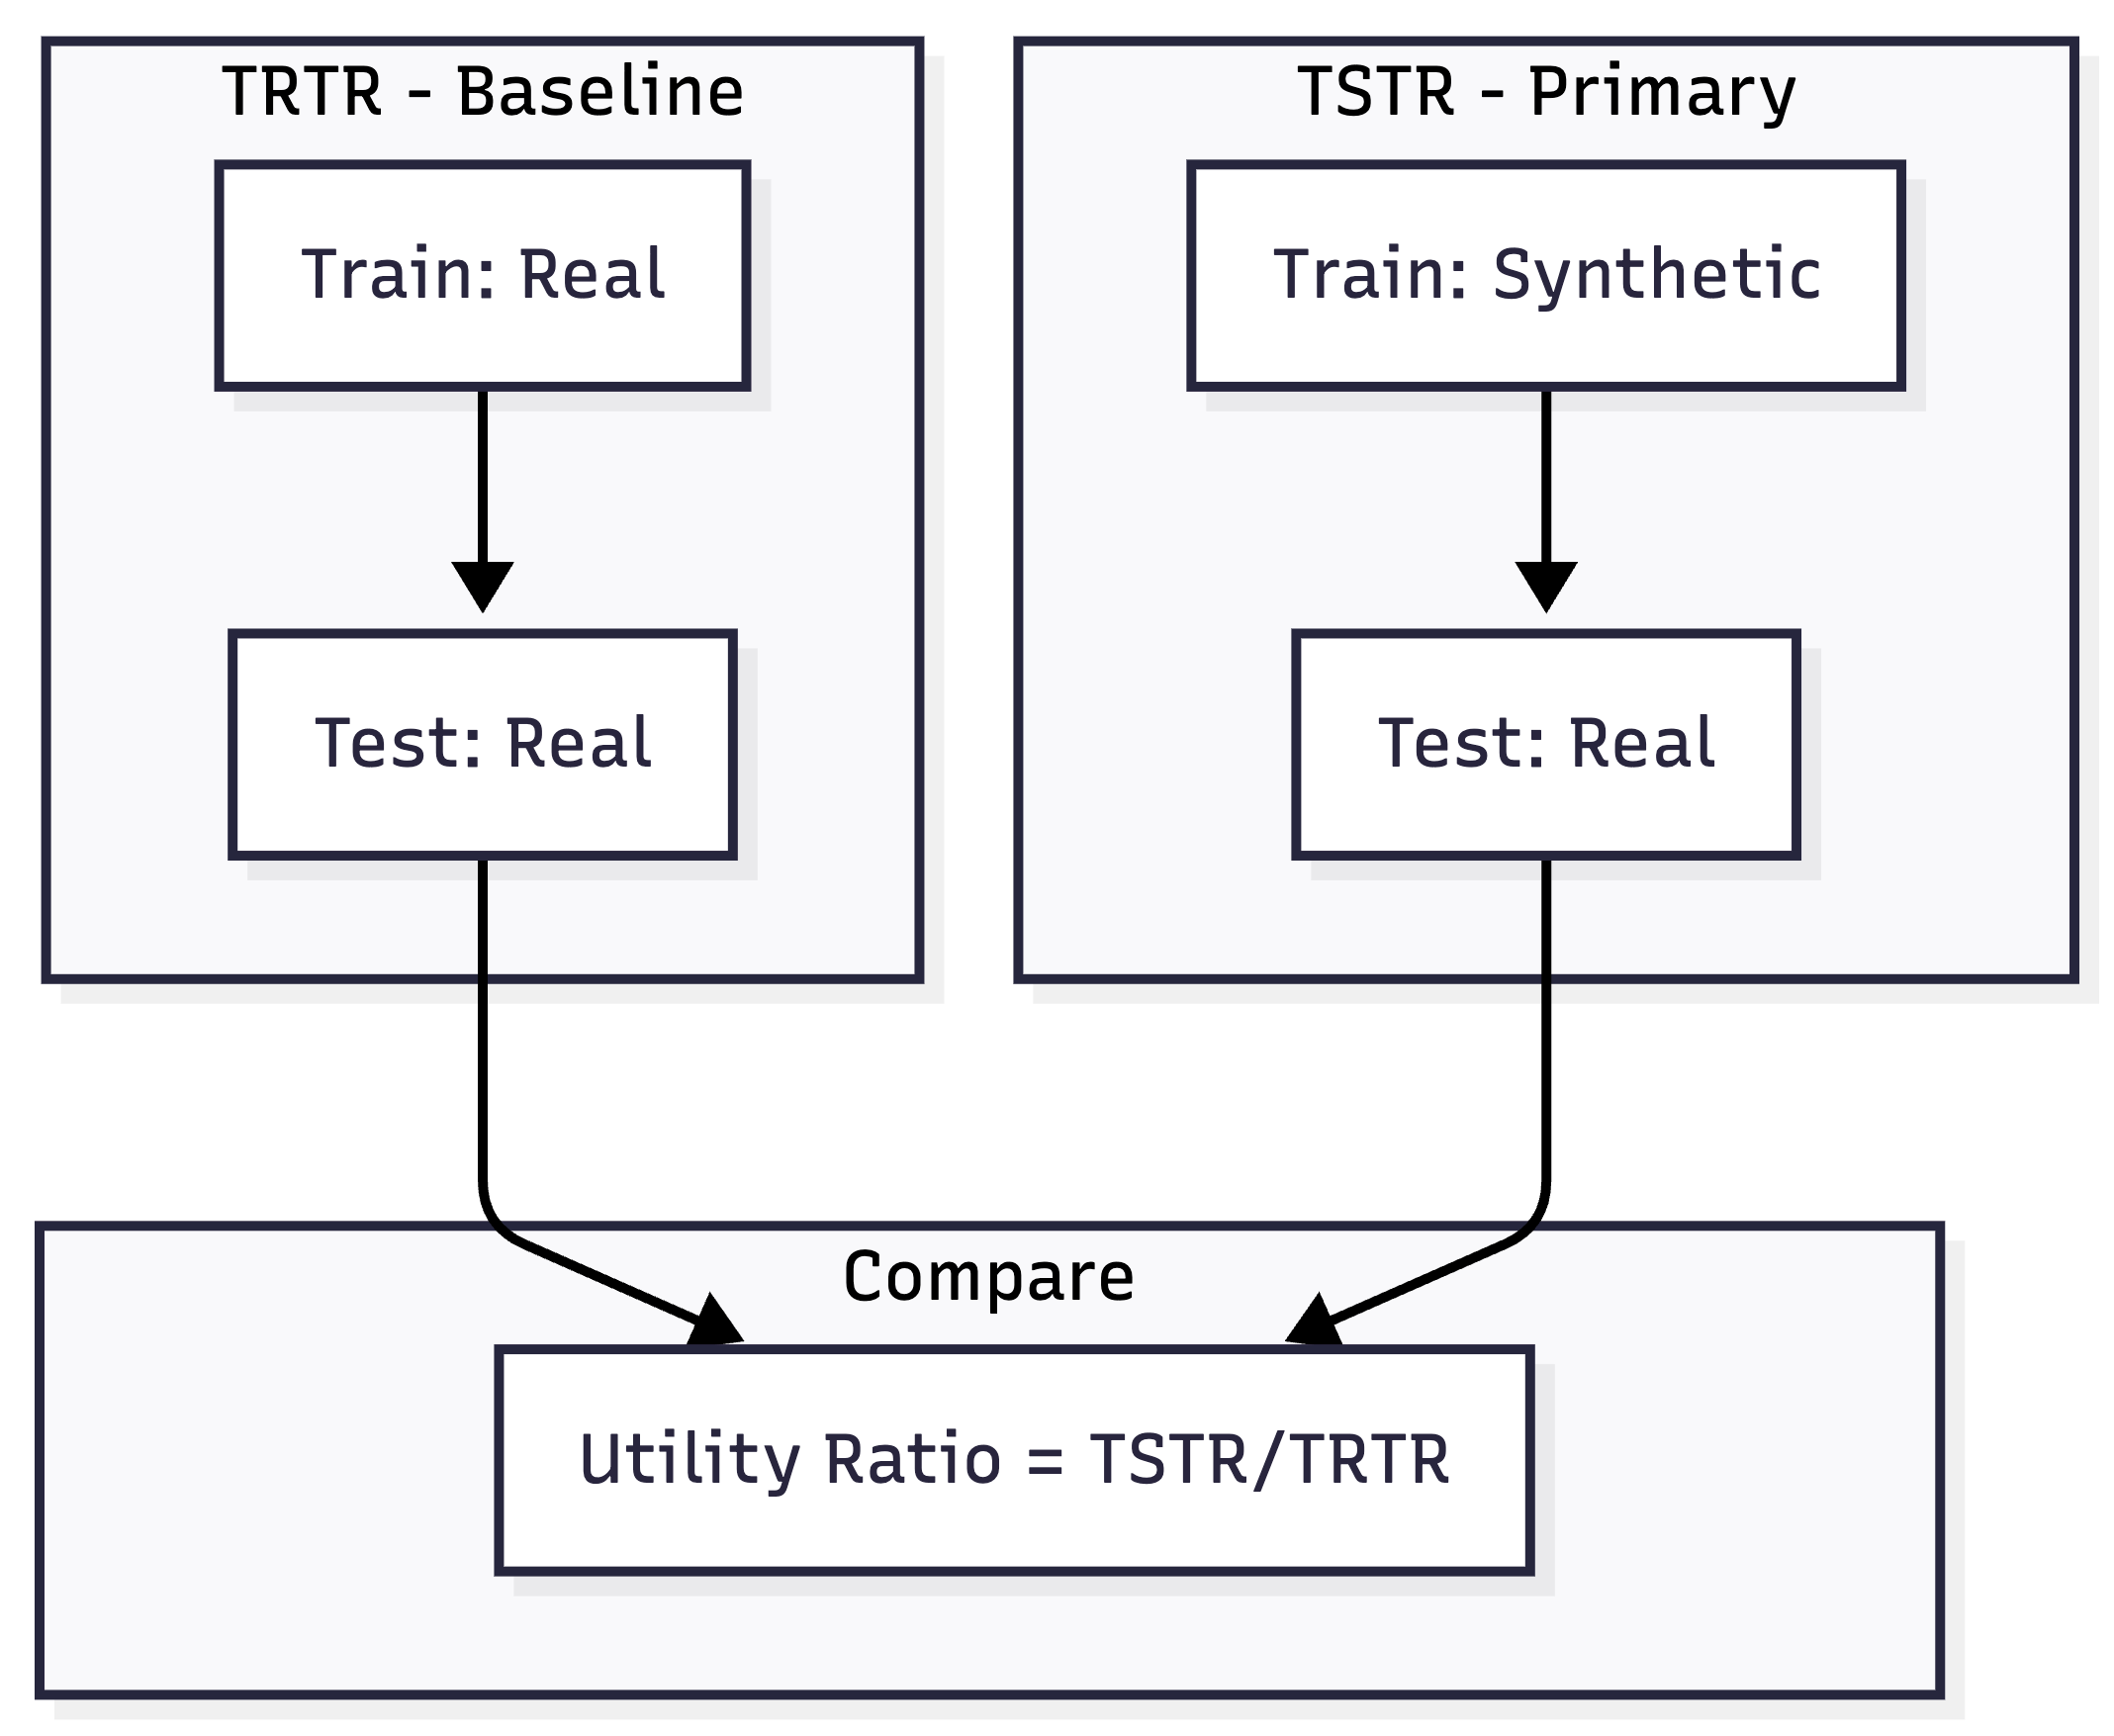
\includegraphics[width=\textwidth]{img/tstr_trtr.png}
\caption{TSTR vs.\ TRTR: utility ratio (TSTR AUC / TRTR AUC) measures how much predictive signal the synthetic data retains.}
\label{fig:tstr_trtr}
\end{figure}

\textbf{TSTR AUC-ROC:} An XGBoost \cite{chen2016xgboost} classifier is trained exclusively on synthetic data (no real training data is used) and evaluated on the real held-out test set. AUC-ROC (Area Under the Receiver Operating Characteristic Curve) measures discrimination ability across all classification thresholds. A value of 0.5 indicates random guessing; a value of 1.0 indicates perfect classification. The TSTR protocol is the most demanding utility test: it asks whether the synthetic data is informative enough to train a fully functional classifier, not merely whether it looks statistically similar.

The XGBoost hyperparameters are fixed across all experiments (learning rate 0.1, 100 estimators, max depth 6) to ensure fair comparison across synthetic data methods. Any performance differences between methods reflect differences in synthetic data quality, not differences in classifier tuning.

\textbf{Minority F1-Score:} The F1-score specifically for the minority class, computed under the TSTR protocol:
\[
F1_{minority} = \frac{2 \cdot \text{Precision}_{minority} \cdot \text{Recall}_{minority}}{\text{Precision}_{minority} + \text{Recall}_{minority}}
\]

This is the most directly relevant utility metric for imbalanced tasks. Precision for the minority class measures: of all records the classifier flagged as minority events, what fraction were actually minority events? Recall measures: of all actual minority events, what fraction did the classifier catch? F1 is their harmonic mean, which is low unless both are high. A model that flags everything as minority has high recall but zero precision (and low F1); a model that flags nothing has neither. F1 captures this balance.

For fraud detection and similar applications, recall (catching actual fraud) is often more important than precision (avoiding false alarms). The F1 metric provides a balanced assessment. In practice, fraud teams might use recall-optimized thresholds, but F1 at the default threshold provides a standardized comparison point.

\subsection{Pillar 3: Privacy preservation}

\begin{figure}[!ht]
\centering
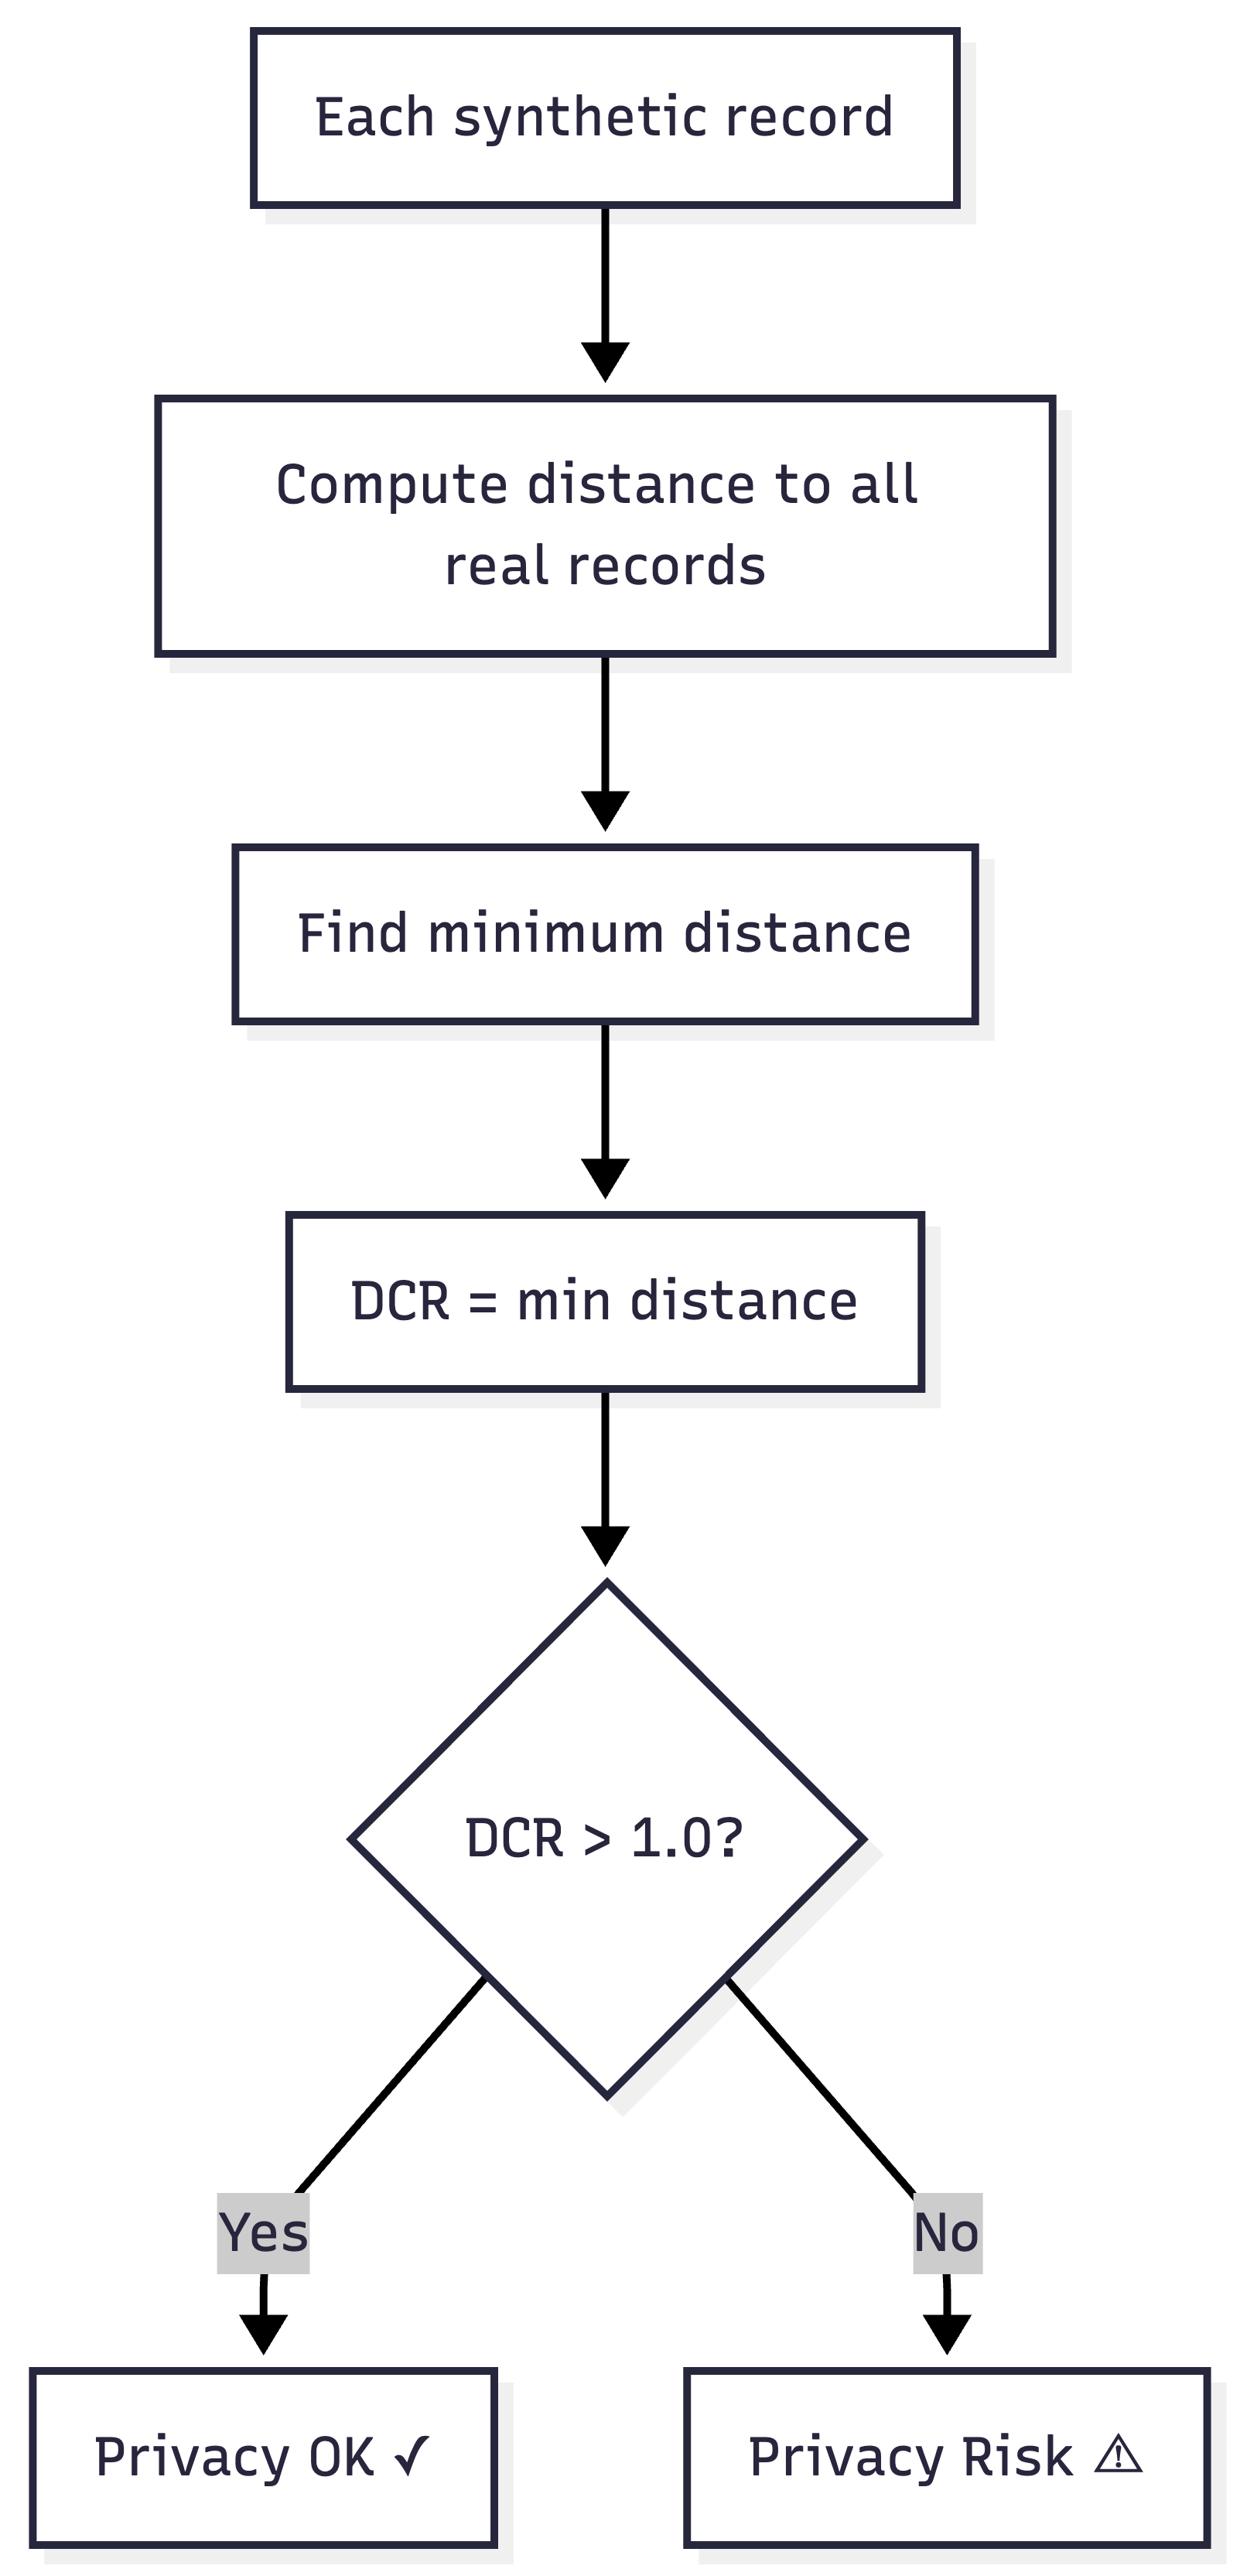
\includegraphics[width=0.65\textwidth]{img/dcr_flowchart.png}
\caption{DCR computation: minimum distance to any real training record; DCR $> 1.0$ is privacy-safe, DCR $\leq 1.0$ flags a memorisation risk.}
\label{fig:dcr_flowchart}
\end{figure}

\textbf{Distance to Closest Record, i.e., DCR:} For each synthetic sample $\tilde{\mathbf{x}}_i$, compute the Euclidean distance to the nearest real training sample:
\[
\text{DCR}(\tilde{\mathbf{x}}_i) = \min_{j} \|\tilde{\mathbf{x}}_i - \mathbf{x}_j\|_2
\]

We report both mean DCR (average privacy across all synthetic samples) and minimum DCR (worst-case privacy). A low minimum DCR indicates that at least one synthetic sample is very close to a real training record, which could represent a privacy risk in settings where the training data is sensitive. A high mean DCR indicates that synthetic samples are generally far from real records, suggesting the model is generating new samples rather than memorizing its training data.

Higher DCR values indicate better empirical privacy. The intuition: if a synthetic record is a near-duplicate of a real record, an adversary who obtains the synthetic data can infer information about the real individual it resembles. If synthetic records are always far from real records, no such inference is possible.

All metrics are computed independently for each of the three random seeds (42, 123, 456), and results are reported as mean $\pm$ standard deviation. This allows assessment of whether performance differences between methods are consistent (low standard deviation) or variable (high standard deviation). A difference between two methods is more credible when it holds across all three seeds than when it is large in one seed and reversed in another.
